%%%%%%%%%%%%%%%%%%%%%%%%%%%%%%%%%%%%%%%%%%%%%%%%%%%%%%%%%%%%%%%%%%%%%%%%%%%%%%%%
%  Zawartość: Główny plik szablonu pracy dyplomowej (magisterskiej/inżynierskiej). 
%  Opracował: Tomasz Kubik <tomasz.kubik@pwr.edu.pl>
%  Data: styczeń 2023
%  Wersja: 0.9
%  Wymagania: kompilator pdflatex
%%%%%%%%%%%%%%%%%%%%%%%%%%%%%%%%%%%%%%%%%%%%%%%%%%%%%%%%%%%%%%%%%%%%%%%%%%%%%%%%

\documentclass[a4paper,onecolumn,oneside,12pt,extrafontsizes]{memoir}
%  W celu przygotowania wydruku do archiwum można:
%  a) przygotować pdf, w którym dwie strony zostaną wstawione na jedną fizyczną stronę i taki dokument wydrukować dwustronnie (podejście zalecane)
%
%   Taki dokument można przygotować poprzez
%   - wydruk z Adobe Acrobat Reader z opcją "Wiele" - sekcja "Rozmiar i obsługa stron"
%   - wykorzystanie narzędzi psutils
%
%      Windows (zakładając, że w dystrybucji MiKTeX jest pakiet miktex-psutils-bin-x64-2.9):
%        "c:\Program Files\MiKTeX 2.9\miktex\bin\x64\pdf2ps.exe" Dyplom.pdf Dyplom.ps
%        "c:\Program Files\MiKTeX 2.9\miktex\bin\x64\psnup.exe" -2 Dyplom.ps Dyplom2.ps
%        "c:\Program Files\MiKTeX 2.9\miktex\bin\x64\ps2pdf.exe" Dyplom2.ps Dyplom2.pdf
%        Del Dyplom2.ps Dyplom.ps
%
%     Linux:
%        pdf2ps Dyplom.pdf - | psnup -2 | ps2pdf - Dyplom2.pdf
%
%  b) przekomplilować dokument zmniejszając czcionkę (podejście niezalecane, bo zmienia formatowanie dokumentu)
%
%    Do tego wystarczy posłużyć się poniższymi komendami (zamiast documentclass z pierwszej linijki):
%   \documentclass[a4paper,onecolumn,twoside,10pt]{memoir} 
%   \renewcommand{\normalsize}{\fontsize{8pt}{10pt}\selectfont}

%\usepackage[cp1250]{inputenc} % Proszę zostawić, jeśli kodowanie edytowanych plików to cp1250 
\usepackage[utf8]{inputenc} % Proszę użyć zamiast powyższego, jeśli kodowanie edytowanych plików to UTF8
\usepackage[T1]{fontenc}
\usepackage[english,polish]{babel} % Tutaj ważna jest kolejność atrybutów (dla pracy po polsku polish powinno być na końcu)
%\DisemulatePackage{setspace}
\usepackage{setspace}
\usepackage{color,calc}
%\usepackage{soul} % pakiet z komendami do podkreślania, przekreślania, podświetlania tekstu (raczej niepotrzebny)
\usepackage{ebgaramond} % pakiet z czcionkami garamond, potrzebny tylko do strony tytułowej, musi wystąpić przed pakietem tgtermes
\usepackage{float}

%% Aby uzyskać polskie literki w pdfie (a nie zlepki) korzystamy z pakietu czcionek tgterms. 
%% W pakiecie tym są zdefiniowane klony czcionek Times o kształtach: normalny, pogrubiony, italic, italic pogrubiony.
%% W pakiecie tym brakuje czcionki o kształcie: slanted (podobny do italic). 
%% Jeśli w dokumencie gdzieś zostanie zastosowana czcionka slanted (np. po użyciu komendy \textsl{}), to
%% latex dokona podstawienia na czcionkę standardową i zgłosi to w ostrzeżeniu (warningu).
%% Ponadto tgtermes to czcionka do tekstu. Wszelkie matematyczne wzory będą sformatowane domyślną czcionką do wzorów.
%% Jeśli wzory mają być sformatowane z wykorzystaniem innych czcionek, trzeba to jawnie zadeklarować.

%% Po zainstalowaniu pakietu tgtermes może będzie trzeba zauktualizować informacje 
%% o dostępnych fontach oraz mapy. Można to zrobić z konsoli (jako administrator)
%% initexmf --admin --update-fndb
%% initexmf --admin --mkmaps

\usepackage{tgtermes}   
\renewcommand*\ttdefault{txtt}


%%%%%%%%%%%%%%%%%%%%%%%%%%%%%%%%%%%%%%%%%%%%%%%%%%%%%%%%%%%%%%%%%%%%%%%%%%%%%%%%
%% Ustawienia odpowiedzialne za sposób łamania dokumentu
%% i ułożenie elementów pływających
%%%%%%%%%%%%%%%%%%%%%%%%%%%%%%%%%%%%%%%%%%%%%%%%%%%%%%%%%%%%%%%%%%%%%%%%%%%%%%%%
%\hyphenpenalty=10000		% nie dziel wyrazów zbyt często
\clubpenalty=10000      % kara za sierotki
\widowpenalty=10000     % nie pozostawiaj wdów
%\brokenpenalty=10000		% nie dziel wyrazów między stronami - trzeba było wyłączyć, bo nie łamały się linie w lstlisting
%\exhyphenpenalty=999999		% nie dziel słów z myślnikiem - trzeba było wyłączyć, bo nie łamały się linie w lstlisting
\righthyphenmin=3			  % dziel minimum 3 litery

%\tolerance=4500
%\pretolerance=250
%\hfuzz=1.5pt
%\hbadness=1450

\renewcommand{\topfraction}{0.95}
\renewcommand{\bottomfraction}{0.95}
\renewcommand{\textfraction}{0.05}
\renewcommand{\floatpagefraction}{0.35}

%%%%%%%%%%%%%%%%%%%%%%%%%%%%%%%%%%%%%%%%%%%%%%%%%%%%%%%%%%%%%%%%%%%%%%%%%%%%%%%%
%%  Ustawienia rozmiarów: tekstu, nagłówka i stopki, marginesów
%%  dla dokumentów klasy memoir 
%%%%%%%%%%%%%%%%%%%%%%%%%%%%%%%%%%%%%%%%%%%%%%%%%%%%%%%%%%%%%%%%%%%%%%%%%%%%%%%%
\setlength{\headsep}{10pt} 
\setlength{\headheight}{13.6pt} % wartość baselineskip dla czcionki 11pt tj. \small wynosi 13.6pt
\setlength{\footskip}{\headsep+\headheight}
\setlength{\uppermargin}{\headheight+\headsep+1cm}
\setlength{\textheight}{\paperheight-\uppermargin-\footskip-1.5cm}
\setlength{\textwidth}{\paperwidth-5cm}
\setlength{\spinemargin}{2.5cm}
\setlength{\foremargin}{2.5cm}
\setlength{\marginparsep}{2mm}
\setlength{\marginparwidth}{2.3mm}
%\settrimmedsize{297mm}{210mm}{*}
%\settrims{0mm}{0mm}	
\checkandfixthelayout[fixed] % konieczne, aby się dobrze wszystko poustawiało
%%%%%%%%%%%%%%%%%%%%%%%%%%%%%%%%%%%%%%%%%%%%%%%%%%%%%%%%%%%%%%%%%%%%%%%%%%%%%%%%
%%  Ustawienia odległości linii, wcięć, odstępów
%%%%%%%%%%%%%%%%%%%%%%%%%%%%%%%%%%%%%%%%%%%%%%%%%%%%%%%%%%%%%%%%%%%%%%%%%%%%%%%%
\linespread{1}
%\linespread{1.241}
\setlength{\parindent}{14.5pt}


\usepackage{multicol} % pakiet umożliwiający stworzenie wielokolumnowego tekstu
%%%%%%%%%%%%%%%%%%%%%%%%%%%%%%%%%%%%%%%%%%%%%%%%%%%%%%%%%%%%%%%%%%%%%%%%%%%%%%%%
%% Pakiety do formatowania tabel
%%%%%%%%%%%%%%%%%%%%%%%%%%%%%%%%%%%%%%%%%%%%%%%%%%%%%%%%%%%%%%%%%%%%%%%%%%%%%%%%
\usepackage{tabularx}
% Proszę używać tylko tabularx. Innych pakietów proszę nie stosować !!!
% Dokument na pewno da się zredagować bez ich użycia.
%\usepackage{longtable}
%\usepackage{ltxtable}
%\usepackage{tabulary}

%%%%%%%%%%%%%%%%%%%%%%%%%%%%%%%%%%%%%%%%%%%%%%%%%%%%%%%%%%%%%%%%%%%%%%%%%%%%%%%%
%% Pakiet do wstawiania fragmentów kodu
%%%%%%%%%%%%%%%%%%%%%%%%%%%%%%%%%%%%%%%%%%%%%%%%%%%%%%%%%%%%%%%%%%%%%%%%%%%%%%%%
\usepackage{listings} 
\usepackage{xpatch}
\makeatletter
\xpatchcmd\l@lstlisting{1.5em}{0em}{}{}
\makeatother
% Pakiet dostarcza otoczenia lstlisting. Jest ono wysoce konfigurowalne. 
% Konfigurować można indywidualnie każdy z listingów lub globalnie, w poleceniu \lstset{}.

% Zalecane jest, by kod źródłowy był wyprowadzany z użyciem czcionki maszynowej \ttfamily
% Ponieważ kod źródłowy, nawet po obcięciu do interesujących fragmentów, bywa obszerny, należy zmniejszyć czcionkę.
% Zalecane jest \small (dla krótkich fragmentów) oraz \footnotesize (dla dłuższych fragmentów).

% Ponadto podczas konfiguracji można zadeklarować sposób numerowania linii. Numerowanie linii zalecane jest jednak 
% tylko w przypadkach, gdy w redagowanym tekście znajdują się jakieś odwołania do konkretnych linii.
% Jeśli takich odwołań nie ma, numerowanie linii jest zbędne. Proszę wtedy go nie stosować.
% Przy włączaniu numerowania linii należy zwrócić uwagę na to, gdzie pojawią się te numery.
% Bez zmiany dodatkowych parametrów pojawiają się one na marginesie strony (co jest niepożądane).

\lstset{
  basicstyle=\small\ttfamily, % lub basicstyle=\footnotesize\ttfamily
  %%columns=fullflexible,
	%%showstringspaces=false,
	%%showspaces=false,
  breaklines=true,
  postbreak=\mbox{\textcolor{red}{$\hookrightarrow$}\space}, 
  %%numbers=left,  % ta i poniższe linie dotyczą ustawienia numerowania i sposobu jego wyprowadzania
  %%firstnumber=1, 
  %%numberfirstline=true, 
	%%xleftmargin=17pt,
  %%framexleftmargin=17pt,
  %%framexrightmargin=5pt,
  %%framexbottommargin=4pt,
	belowskip=.5\baselineskip,
	literate={\_}{{\_\allowbreak}}1 % ta deklaracja przydaje się, jeśli na listingu mają być łamane nazwy zawierające podkreślniki
}

% Jeśli edytowany plik nie jest w kodowaniu cp1250, to jest problem z polskimi znakami występującymi we wstawianym kodzie.
% Dlatego podczas pracy na plikach w kodowaniu UTF8 trzeba zadeklarować mapowanie jak niżej (wystarczy odmarkować).
% Niestety, jak się zastosuje to mapowanie mogą pojawić się problemy z podświetlaniem składni (patrz dalej).
\lstset{literate=%-
{ą}{{\k{a}}}1 {ć}{{\'c}}1 {ę}{{\k{e}}}1 {ł}{{\l{}}}1 {ń}{{\'n}}1 {ó}{{\'o}}1 {ś}{{\'s}}1 {ż}{{\.z}}1 {ź}{{\'z}}1 {Ą}{{\k{A}}}1 {Ć}{{\'C}}1 {Ę}{{\k{E}}}1 {Ł}{{\L{}}}1 {Ń}{{\'N}}1 {Ó}{{\'O}}1 {Ś}{{\'S}}1 {Ż}{{\.Z}}1 {Ź}{{\'Z}}1 
    {Ö}{{\"O}}1
    {Ä}{{\"A}}1
    {Ü}{{\"U}}1
    {ß}{{\ss}}1
    {ü}{{\"u}}1
    {ä}{{\"a}}1
    {ö}{{\"o}}1
    {~}{{\textasciitilde}}1
		{—}{{{\textemdash} }}1
}%{\ \ }{{\ }}1}


%% lstlisting pozwala na ostylowania podświetlania składni wybranych języków.
%% Działa to na zasadzie zdefiniowania słów kluczowych oraz sposobu ich wyświetlania.
%% Ponieważ jest to prosty mechanizm, czasem trudno osiągnąć takie efekty, jakie dają narzędzia IDE. 
%% Jednak w większości przypadku osiągane rezutlaty są zadowalające.


%% lstlisting obsługuje domyślnie kilka najpopularniejszych języków.
%%\lstloadlanguages{% Check Dokumentation for further languages ...
%%C,
%%C++,
%%csh,
%%Java
%%}
%% Inne języki muszą być dodefiniowane. Poniżej podano przykłady definicji języków i styli.

\definecolor{lightgray}{rgb}{.9,.9,.9}
\definecolor{darkgray}{rgb}{.4,.4,.4}
\definecolor{purple}{rgb}{0.65, 0.12, 0.82}
\definecolor{javared}{rgb}{0.6,0,0} % for strings
\definecolor{javagreen}{rgb}{0.25,0.5,0.35} % comments
\definecolor{javapurple}{rgb}{0.5,0,0.35} % keywords
\definecolor{javadocblue}{rgb}{0.25,0.35,0.75} % javadoc
 
\lstdefinelanguage{JavaScript}{ 
	keywords={typeof, new, true, false, catch, function, return, null, catch, switch, var, if, in, while, do, else, case, break},
	keywordstyle=\color{blue}\bfseries,
	ndkeywords={class, export, boolean, throw, implements, import, this},
	ndkeywordstyle=\color{darkgray}\bfseries,
	identifierstyle=\color{black},
	sensitive=false,
	comment=[l]{//},
	morecomment=[s]{/*}{*/},
	commentstyle=\color{purple}\ttfamily,
	stringstyle=\color{red}\ttfamily,
	morestring=[b]',
	morestring=[b]"
}
\lstdefinestyle{JavaScriptStyle}{
	language=JavaScript,
	commentstyle=\color{javagreen}, % niestety, jeśli w linii komentarza pojawią się słowa kluczowe, to zostaną pokolorowane
	backgroundcolor=,%\color{lightgray}, % można ustwić kolor tła, ale jest to niezalecane
	extendedchars=true,
	basicstyle=\footnotesize\ttfamily,
	showstringspaces=false,
	showspaces=false,
	numbers=none,%left,
	numberstyle=\footnotesize,
	numbersep=9pt,
	tabsize=2,
	breaklines=true,
	showtabs=false,
	captionpos=t
}

\lstdefinestyle{JavaStyle}{
basicstyle=\footnotesize\ttfamily,
keywordstyle=\color{javapurple}\bfseries,
stringstyle=\color{javared},
commentstyle=\color{javagreen},
morecomment=[s][\color{javadocblue}]{/**}{*/},
numbers=none,%left,
numberstyle=\tiny\color{black},
stepnumber=2,
numbersep=10pt,
tabsize=4,
showspaces=false,
showstringspaces=false,
captionpos=t
}

\definecolor{pblue}{rgb}{0.13,0.13,1}
\definecolor{pgreen}{rgb}{0,0.5,0}
\definecolor{pred}{rgb}{0.9,0,0}
\definecolor{pgrey}{rgb}{0.46,0.45,0.48}
\definecolor{dark-grey}{rgb}{0.4,0.4,0.4}
% styl json
\newcommand\JSONnumbervaluestyle{\color{blue}}
\newcommand\JSONstringvaluestyle{\color{red}}

\newif\ifcolonfoundonthisline

\makeatletter

\lstdefinestyle{json-style}  
{
	showstringspaces    = false,
	keywords            = {false,true},
	alsoletter          = 0123456789.,
	morestring          = [s]{"}{"},
	stringstyle         = \ifcolonfoundonthisline\JSONstringvaluestyle\fi,
	MoreSelectCharTable =%
	\lst@DefSaveDef{`:}\colon@json{\processColon@json},
	basicstyle          = \footnotesize\ttfamily,
	keywordstyle        = \ttfamily\bfseries,
	numbers				= left, % zakomentować, jeśli numeracja linii jest niepotrzebna
	numberstyle={\footnotesize\ttfamily\color{dark-grey}},
	xleftmargin			= 2em % zakomentować, jeśli numeracja linii jest niepotrzebna
}

\newcommand\processColon@json{%
	\colon@json%
	\ifnum\lst@mode=\lst@Pmode%
	\global\colonfoundonthislinetrue%
	\fi
}

\lst@AddToHook{Output}{%
	\ifcolonfoundonthisline%
	\ifnum\lst@mode=\lst@Pmode%
	\def\lst@thestyle{\JSONnumbervaluestyle}%
	\fi
	\fi
	\lsthk@DetectKeywords% 
}

\lst@AddToHook{EOL}%
{\global\colonfoundonthislinefalse}

\makeatother

%%\definecolor{red}{rgb}{0.6,0,0} % for strings
%%\definecolor{blue}{rgb}{0,0,0.6}
%%\definecolor{green}{rgb}{0,0.8,0}
%%\definecolor{cyan}{rgb}{0.0,0.6,0.6}
%%
%%\lstdefinestyle{sqlstyle}{
%%language=SQL,
%%basicstyle=\footnotesize\ttfamily, 
%%numbers=left, 
%%numberstyle=\tiny, 
%%numbersep=5pt, 
%%tabsize=2, 
%%extendedchars=true, 
%%breaklines=true, 
%%showspaces=false, 
%%showtabs=true, 
%%xleftmargin=17pt,
%%framexleftmargin=17pt,
%%framexrightmargin=5pt,
%%framexbottommargin=4pt,
%%keywordstyle=\color{blue}, 
%%commentstyle=\color{green}, 
%%stringstyle=\color{red}, 
%%}
%%
%%\lstdefinestyle{sharpcstyle}{
%%language=[Sharp]C,
%%basicstyle=\footnotesize\ttfamily, 
%%numbers=left, 
%%numberstyle=\tiny, 
%%numbersep=5pt, 
%%tabsize=2, 
%%extendedchars=true, 
%%breaklines=true, 
%%showspaces=false, 
%%showtabs=true, 
%%xleftmargin=17pt,
%%framexleftmargin=17pt,
%%framexrightmargin=5pt,
%%framexbottommargin=4pt,
%%morecomment=[l]{//}, %use comment-line-style!
%%morecomment=[s]{/*}{*/}, %for multiline comments
%%showstringspaces=false, 
%%morekeywords={  abstract, event, new, struct,
                %%as, explicit, null, switch,
                %%base, extern, object, this,
                %%bool, false, operator, throw,
                %%break, finally, out, true,
                %%byte, fixed, override, try,
                %%case, float, params, typeof,
                %%catch, for, private, uint,
                %%char, foreach, protected, ulong,
                %%checked, goto, public, unchecked,
                %%class, if, readonly, unsafe,
                %%const, implicit, ref, ushort,
                %%continue, in, return, using,
                %%decimal, int, sbyte, virtual,
                %%default, interface, sealed, volatile,
                %%delegate, internal, short, void,
                %%do, is, sizeof, while,
                %%double, lock, stackalloc,
                %%else, long, static,
                %%enum, namespace, string},
%%keywordstyle=\color{cyan},
%%identifierstyle=\color{red},
%%stringstyle=\color{blue}, 
%%commentstyle=\color{green},
%%}



%%%%%%%%%%%%%%%%%%%%%%%%%%%%%%%%%%%%%%%%%%%%%%%%%%%%%%%%%%%%%%%%%%%%%%%%%%%%%%%%
%%  Pakiety i komendy zastosowane tylko do zamieszczenia informacji o użytych komendach i fontach w tym szablonie.
%%  Normalnie nie są one potrzebne. Proszę poniższe deklaracje zamarkować podczas redakcji pracy !!!!
%%%%%%%%%%%%%%%%%%%%%%%%%%%%%%%%%%%%%%%%%%%%%%%%%%%%%%%%%%%%%%%%%%%%%%%%%%%%%%%%
%%\usepackage{memlays}     % extra layout diagrams, zastosowane w szblonie do 'debuggowania', używa pakietu layouts
%\usepackage{layouts}
%%\usepackage{printlen} % pakiet do wyświetlania wartości zdefiniowanych długości, stosowany do 'debuggowania'
%%\usepackage{enumitem} % pakiet do numerowania 1.1 1.2 w sekcji enumrate
%%\uselengthunit{pt}
%%\makeatletter
%%\newcommand{\showFontSize}{\f@size pt} % makro wypisujące wielkość bieżącej czcionki
%%\makeatother
% do pokazania ramek można byłoby użyć:
%\usepackage{showframe} 

%%%%%%%%%%%%%%%%%%%%%%%%%%%%%%%%%%%%%%%%%%%%%%%%%%%%%%%%%%%%%%%%%%%%%%%%%%%%%%%%
%%  Formatowanie list wyliczeniowych, wypunktowań i własnych otoczeń
%%%%%%%%%%%%%%%%%%%%%%%%%%%%%%%%%%%%%%%%%%%%%%%%%%%%%%%%%%%%%%%%%%%%%%%%%%%%%%%%

% Domyślnie wypunktowania mają zadeklarowane znaki, które nie występują w tgtermes
% Aby latex nie podstawiał w ich miejsca znaków z czcionki standardowej można zrobić podstawienie:
%    \DeclareTextCommandDefault{\textbullet}{\ensuremath{\bullet}}
%    \DeclareTextCommandDefault{\textasteriskcentered}{\ensuremath{\ast}}
%    \DeclareTextCommandDefault{\textperiodcentered}{\ensuremath{\cdot}}
% Jednak jeszcze lepszym pomysłem jest zdefiniowanie otoczeń z wykorzystaniem enumitem
\usepackage{enumitem} % pakiet pozwalający zarządzać formatowaniem list wyliczeniowych
\setlist{noitemsep,topsep=4pt,parsep=0pt,partopsep=4pt,leftmargin=*} % zadeklarowane parametry pozwalają uzyskać 'zwartą' postać wypunktowania bądź wyliczenia
\setenumerate{labelindent=0pt,itemindent=0pt,leftmargin=!,label=\arabic*.} % można zmienić \arabic na \alph, jeśli wyliczenia mają być z literkami
\setlistdepth{4} % definiujemy głębokość zagnieżdżenia list wyliczeniowych do 4 poziomów
\setlist[itemize,1]{label=$\bullet$}  % definiujemy, jaki symbol ma być użyty w wyliczeniu na danym poziomie
\setlist[itemize,2]{label=\normalfont\bfseries\textendash}
\setlist[itemize,3]{label=$\ast$}
\setlist[itemize,4]{label=$\cdot$}
\renewlist{itemize}{itemize}{4}

%%%http://tex.stackexchange.com/questions/29322/how-to-make-enumerate-items-align-at-left-margin
%\renewenvironment{enumerate}
%{
%\begin{list}{\arabic{enumi}.}
%{
%\usecounter{enumi}
%%\setlength{\itemindent}{0pt}
%%\setlength{\leftmargin}{1.8em}%{2zw} % 
%%\setlength{\rightmargin}{0zw} %
%%\setlength{\labelsep}{1zw} %
%%\setlength{\labelwidth}{3zw} % 
%\setlength{\topsep}{6pt}%
%\setlength{\partopsep}{0pt}%
%\setlength{\parskip}{0pt}%
%\setlength{\parsep}{0em} % 
%\setlength{\itemsep}{0em} % 
%%\setlength{\listparindent}{1zw} % 
%}
%}{
%\end{list}
%}

\makeatletter
\renewenvironment{quote}{
	\begin{list}{}
	{
	\setlength{\leftmargin}{1em}
	\setlength{\topsep}{0pt}%
	\setlength{\partopsep}{0pt}%
	\setlength{\parskip}{0pt}%
	\setlength{\parsep}{0pt}%
	\setlength{\itemsep}{0pt}
	}
	}{
	\end{list}}
\makeatother

%%%%%%%%%%%%%%%%%%%%%%%%%%%%%%%%%%%%%%%%%%%%%%%%%%%%%%%%%%%%%%%%%%%%%%%%%%%%%%%%
%%  Pakiet i komendy do generowania indeksu 
%% (ważne, by pojawiły się przed pakietem hyperref)
%%%%%%%%%%%%%%%%%%%%%%%%%%%%%%%%%%%%%%%%%%%%%%%%%%%%%%%%%%%%%%%%%%%%%%%%%%%%%%%%
% pdftex jest w stanie wygenerować indeks (czyli spis haseł z referencjami do stron, na których te hasła się pojawiły).
% Generalnie z indeksem jest sporo problemów, zwłaszcza, gdy pojawiają się polskie literki.
% Trzeba wtedy korzystać z xindy.
% Zwykle w pracach dyplomowych indeksy nie są wykorzystywane. Dlatego są zamarkowane.
%\DisemulatePackage{imakeidx}
%\usepackage[makeindex,noautomatic]{imakeidx} % tutaj mówimy, żeby indeks nie generował się automatycznie, 
%\makeindex
%
%\makeatletter
%%%%\renewenvironment{theindex}
							 %%%%{\vskip 10pt\@makeschapterhead{\indexname}\vskip -3pt%
								%%%%\@mkboth{\MakeUppercase\indexname}%
												%%%%{\MakeUppercase\indexname}%
								%%%%\vspace{-3.2mm}\parindent\z@%
								%%%%\renewcommand\subitem{\par\hangindent 16\p@ \hspace*{0\p@}}%%
								%%%%\phantomsection%
								%%%%\begin{multicols}{2}
								%%%%%\thispagestyle{plain}
								%%%%\parindent\z@                
								%%%%%\parskip\z@ \@plus .3\p@\relax
								%%%%\let\item\@idxitem}
							 %%%%{\end{multicols}\clearpage}
%%%%
%\makeatother




%%%%%%%%%%%%%%%%%%%%%%%%%%%%%%%%%%%%%%%%%%%%%%%%%%%%%%%%%%%%%%%%%%%%%%%%%%%%%%%%
%%  Sprawy metadanych w wynikowym pdf, hyperlinków itp.
%%%%%%%%%%%%%%%%%%%%%%%%%%%%%%%%%%%%%%%%%%%%%%%%%%%%%%%%%%%%%%%%%%%%%%%%%%%%%%%%
% Szablon przygotowano głównie dla pdflatex. Specyficzne komendy dla pdf-owej kompilacj wstawiono 
% w instrukcję warunkową dostarczaną przez pakiet ifpdf 
% Jeśli metadane zawierają przecinki lub średniki, domyślnie metadane te otaczane są apostrofami.
% Piszą o tym na stronie: https://tex.stackexchange.com/questions/3708/hyperref-enquotes-metadata
% Aby pozbyć się tych apostrofów użyto pakietu hyperxmp (ładującego kilka innych pakietów)
\usepackage{hyperxmp}
\usepackage{ifpdf}
%\newif\ifpdf \ifx\pdfoutput\undefined
%\pdffalse % we are not running PDFLaTeX
%\else
%\pdfoutput=1 % we are running PDFLaTeX
%\pdftrue \fi
\ifpdf
 \usepackage{datetime2} % INFO: pakiet potrzeby do uzyskania i sformatowania daty 
 \usepackage[pdftex,bookmarks,breaklinks,unicode]{hyperref}
 \usepackage[pdftex]{graphicx}
 \DeclareGraphicsExtensions{.pdf,.jpg,.mps,.png} % po zadeklarowaniu rozszerzeń można będzie wstawiać pliki z grafiką bez konieczności podawania tych rozszerzeń w ich nazwach
\pdfcompresslevel=9
\pdfoutput=1

% Dobrze przygotowany dokument pdf to taki, który zawiera metadane.
% Poniżej zadeklarowano pola metadanych, jakie będą włączone do dokumentu pdf.
% Można je zmodyfikować w zależności od potrzeb
\makeatletter
\AtBeginDocument{  
  \hypersetup{
	pdfinfo={
    Title = {\@title},
    Author = {\@author},
    Subject={Praca dyplomowa \ifMaster magisterska\else inżynierska\fi},  
    Keywords={\@kvpl}, 
		Producer={}, 
	  CreationDate= {}, % należy wstawiać zgodnie ze składnią: {D:yyyymmddhhmmss}, np. D:20210208175600
    ModDate={\pdfcreationdate},   % data modyfikacji będzie datą kompilacji
		Creator={pdftex},
	}}
}
\pdftrailerid{} %Remove ID
\pdfsuppressptexinfo15 %Suppress PTEX.Fullbanner and info of imported PDFs
\makeatother
\else             % jeśli kompilacja jest inna niż pdflatex
\usepackage{graphicx}
\DeclareGraphicsExtensions{.eps,.ps,.jpg,.mps,.png}
\fi
\sloppy

% INFO: dodane by lepiej łamać urle 
\def\UrlBreaks{\do\/\do-\do_} 
% INFO: choć można zadeklarować foldery, w jakich pojawiać się mają pliki z grafiką, zaleca się jednak, by tego nie robić
%\graphicspath{{rys01/}{rys02/}}  


%%%%%%%%%%%%%%%%%%%%%%%%%%%%%%%%%%%%%%%%%%%%%%%%%%%%%%%%%%%%%%%%%%%%%%%%%%%%%%%%
%%  Formatowanie dokumentu
%%%%%%%%%%%%%%%%%%%%%%%%%%%%%%%%%%%%%%%%%%%%%%%%%%%%%%%%%%%%%%%%%%%%%%%%%%%%%%%%
% INFO: Deklaracja głębokościu numeracji
\setcounter{secnumdepth}{2}
\setcounter{tocdepth}{2}
\setsecnumdepth{subsection} 
% INFO: Dodanie kropek po numerach sekcji
\makeatletter
\def\@seccntformat#1{\csname the#1\endcsname.\quad}
\def\numberline#1{\hb@xt@\@tempdima{#1\if&#1&\else.\fi\hfil}}
\makeatother
% INFO: Numeracja rozdziałów i separatory
\renewcommand{\chapternumberline}[1]{#1.\quad}
\renewcommand{\cftchapterdotsep}{\cftdotsep}


%\usepackage{etoolbox} % odstępy w spisie treści (jeden ze sposobów ustawiania)
%%\makeatletter
%%\pretocmd{\chapter}{\addtocontents{toc}{\protect\addvspace{-1\p@}}}{}{}
%%\pretocmd{\section}{\addtocontents{toc}{\protect\addvspace{-1\p@}}}{}{}
%%\pretocmd{\subsection}{\addtocontents{toc}{\protect\addvspace{-1\p@}}}{}{}
%%\makeatother

\makeatletter % odstępy w spisie pomiędzy rozdziałami
\renewcommand*{\insertchapterspace}{%
  \addtocontents{lof}{\protect\addvspace{3pt}}%
  \addtocontents{lot}{\protect\addvspace{3pt}}%
	\addtocontents{toc}{\protect\addvspace{3pt}} %
  \addtocontents{lol}{\protect\addvspace{3pt}}}
\makeatother 


\setlength{\cftbeforechapterskip}{0pt} % odstępy w spisie treści przed rozdziałem, działa w korelacji z:
\renewcommand{\aftertoctitle}{\afterchaptertitle\vspace{-4pt}} % 
% https://stackoverflow.com/questions/3029271/latex-make-listoffigures-look-like-listoftables-or-lstlistoflistings
%\renewcommand{\memchapinfo}[4]{%
%  \addtocontents{lol}{\protect\addvspace{10pt}}
%}

%\cftsetindents{section}{1.5em}{2.3em}

%\setbeforesecskip{10pt plus 0.5ex}%{-3.5ex \@plus -1ex \@minus -.2ex}
%\setaftersecskip{10pt plus 0.5ex}%\onelineskip}
%\setbeforesubsecskip{8pt plus 0.5ex}%{-3.5ex \@plus -1ex \@minus -.2ex}
%\setaftersubsecskip{8pt plus 0.5ex}%\onelineskip}
%\setlength\floatsep{6pt plus 2pt minus 2pt} 
%\setlength\intextsep{12pt plus 2pt minus 2pt} 
%\setlength\textfloatsep{12pt plus 2pt minus 2pt} 

% Ustawienie odstępu od góry w nienumerowanych rozdziałach oraz wykazach:
% Spis treści, Spis tabel, Spis rysunków, Indeks rzeczowy
%\newlength{\linespace}
%\setlength{\linespace}{-\beforechapskip-\topskip+\headheight+\topsep}
%%%\makechapterstyle{noNumbered}{%
%%%\renewcommand\chapterheadstart{\vspace*{\linespace}}
%%%}
%% powyższa komenda załatwia to, co robią komendy poniższe dla spisów
%\renewcommand*{\tocheadstart}{\vspace*{\linespace}}
%\renewcommand*{\lotheadstart}{\vspace*{\linespace}}
%\renewcommand*{\lofheadstart}{\vspace*{\linespace}}


% INFO: Czcionka do podpisów tabel, rysunków, listingów
\captionnamefont{\small}
\captiontitlefont{\small}


% INFO: Sformatowanie podpisu nad dwukolumnowym listingiem
\newcommand{\listingcaption}[1]
{%
\vspace*{\abovecaptionskip}\small 
\refstepcounter{lstlisting}\hfill%
Listing \thelstlisting: #1\hfill%\hfill%
\addcontentsline{lol}{lstlisting}{\protect\numberline{\thelstlisting}#1}
}%



% INFO: Pomocnicze marko do wyróżniania tekstu w języku angielskim
\newcommand{\eng}[1]{(ang.~\emph{#1})}
% IFNO: Pomocnicze makro do dołączania podpisów do rysunków ze wskazaniem źródła (bez wypisywania tego źródła w spisie rysunków)
\newcommand*{\captionsource}[2]{%
  \caption[{#1}]{%
    #1 \emph{Źródło:} #2%
  }%
}


% INFO: Makro pozwalające zmienić sposób wypisywania rozdziału (proszę z niego nie korzystać)
%\def\printchaptertitle##1{\fonttitle \space \thechapter.\space ##1} 

% INFO: definicje etykiet i tytułów spisów

%\AtBeginDocument{% 
        \addto\captionspolish{% 
        \renewcommand{\tablename}{Tab.}%% INFO: Przedefiniowanie etykiet w podpisach tabel 
}%} 

%\AtBeginDocument{% 
%        \addto\captionspolish{% 
%        \renewcommand{\chaptername}{Rozdział}% INFO: Przedefiniowanie nazwy rozdziału, niepotrzebne, bo przy polskich ustawieniach językowych jest 'Rozdział'
%}} 

% Przedefiniowanie etykiet oraz nazw wykazu literatury, spisów, indeksu
%\AtBeginDocument{% 
        \addto\captionspolish{% 
        \renewcommand{\figurename}{Rys.}%% INFO: Przedefiniowanie etykiet w podpisach rysunków 
}%}

%\AtBeginDocument{% 
        \addto\captionspolish{% 
        \renewcommand{\lstlistlistingname}{Spis listingów}%% INFO: Przedefiniowanie nazwy spisu listingów
}%} 
\newlistof{lstlistoflistings}{lol}{\lstlistlistingname}


%\AtBeginDocument{% 
        \addto\captionspolish{% 
        \renewcommand{\bibname}{Literatura}%% INFO: Przedefiniowanie nazwy wykazu literatury 
}%}

%\AtBeginDocument{% 
        \addto\captionspolish{% 
        \renewcommand{\listfigurename}{Spis rysunków}%% INFO: Przedefiniowanie nazwy spisu rysunków 
}%}

%\AtBeginDocument{% 
        \addto\captionspolish{% 
        \renewcommand{\listtablename}{Spis tabel}%% INFO: Przedefiniowanie nazwy spisu tabel 
}%}

%\AtBeginDocument{% 
        \addto\captionspolish{% 
\renewcommand\indexname{Indeks rzeczowy}%% INFO: Przedefiniowanie nazwy indeksu 
}%}

%\AtBeginDocument{% 
%    \addto\captionspolish{
%\renewcommand\abstractname{Streszczenie}%% INFO: Przedefiniowanie nazwy strzeszczenia, niepotrzebne, bo przy polskich ustawieniach językowych jest 'Streszczenie'
%}%}

%\AtBeginDocument{% 
%    \addto\captionsenglish{
%\renewcommand\abstractname{Abstract} 
%}%}

%\let\oldmarkboth\markboth
%\renewcommand{\markboth}[2]{\oldmarkboth{\small{#1}}{\small{#2}}}

\renewcommand{\abstractnamefont}{\normalfont\Large\bfseries}
\renewcommand{\abstracttextfont}{\normalfont}


%%%%%%%%%%%%%%%%%%%%%%%%%%%%%%%%%%%%%%%%%%%%%%%%%%%%%%%%%%%%%%%%%%%%%%%%%%%%%%%%
%% Definicje stopek i nagłówków
%%%%%%%%%%%%%%%%%%%%%%%%%%%%%%%%%%%%%%%%%%%%%%%%%%%%%%%%%%%%%%%%%%%%%%%%%%%%%%%%
\addtopsmarks{headings}{%
\nouppercaseheads % added at the beginning
}{%
\createmark{chapter}{both}{shownumber}{}{. \space}
%\createmark{chapter}{left}{shownumber}{}{. \space}
\createmark{section}{right}{shownumber}{}{. \space}
}%use the new settings

\makeatletter
\copypagestyle{outer}{headings}
\makeoddhead{outer}{}{}{\small\itshape\rightmark}
\makeevenhead{outer}{\small\itshape\leftmark}{}{}
\makeoddfoot{outer}{\small\@author:~\@titleShort}{}{\small\thepage}
\makeevenfoot{outer}{\small\thepage}{}{\small\@author:~\@title}
\makeheadrule{outer}{\linewidth}{\normalrulethickness}
\makefootrule{outer}{\linewidth}{\normalrulethickness}{2pt}
\makeatother

% fix plain
\copypagestyle{plain}{headings} % overwrite plain with outer
\makeoddhead{plain}{}{}{} % remove right header
\makeevenhead{plain}{}{}{} % remove left header
\makeevenfoot{plain}{}{}{}
\makeoddfoot{plain}{}{}{}

\copypagestyle{empty}{headings} % overwrite plain with outer
\makeoddhead{empty}{}{}{} % remove right header
\makeevenhead{empty}{}{}{} % remove left header
\makeevenfoot{empty}{}{}{}
\makeoddfoot{empty}{}{}{}

% INFO: deklaracja zmiennej logicznej wykorzystywanej do rozróżnienia pracy inżynierskiej i magisterskiej
\newif\ifMaster% domyślnie false (czyli domyślnie mamy pracę inżynierską)

%%%%%%%%%%%%%%%%%%%%%%%%%%%%%%%%%%%%%%%%%%%%%%%%%%%%%%%%%%%%%%%%%%%%%%%%%%%%%%%%
%% Definicja strony tytułowej 
%%%%%%%%%%%%%%%%%%%%%%%%%%%%%%%%%%%%%%%%%%%%%%%%%%%%%%%%%%%%%%%%%%%%%%%%%%%%%%%%
\makeatletter
%Uczelnia
\newcommand\uczelnia[1]{\renewcommand\@uczelnia{#1}}
\newcommand\@uczelnia{}
%Wydział
\newcommand\wydzial[1]{\renewcommand\@wydzial{#1}}
\newcommand\@wydzial{}
%Kierunek
\newcommand\kierunek[1]{\renewcommand\@kierunek{#1}}
\newcommand\@kierunek{}
%Specjalność
\newcommand\specjalnosc[1]{\renewcommand\@specjalnosc{#1}}
\newcommand\@specjalnosc{}
%Tytuł po angielsku
\newcommand\titleEN[1]{\renewcommand\@titleEN{#1}}
\newcommand\@titleEN{}
%Tytuł krótki
\newcommand\titleShort[1]{\renewcommand\@titleShort{#1}}
\newcommand\@titleShort{}
%Promotor
\newcommand\promotor[1]{\renewcommand\@promotor{#1}}
\newcommand\@promotor{}
%Słowa kluczowe
\newcommand\kvpl[1]{\renewcommand\@kvpl{#1}}
\newcommand\@kvpl{}
\newcommand\kven[1]{\renewcommand\@kven{#1}}
\newcommand\@kven{}
%Komenda wykorzystywana w streszczeniu
\newcommand\mykeywords{\hspace{\absleftindent}%
\parbox{\linewidth-2.0\absleftindent}{
       \iflanguage{polish}{\textbf{Słowa kluczowe:} \@kvpl}{%
			 \iflanguage{english}{\textbf{Keywords:} \@kven}}{}}
				}

\def\maketitle{%
  \pagestyle{empty}%
%%\garamond 
	\fontfamily{\ebgaramond@family}\selectfont % na stronie tytułowej czcionka garamond
%%%%%%%%%%%%%%%%%%%%%%%%%%%%%%%%%%%%%%%%%%%%%%%%%%%%%%%%%%%%%%%%%%%%%%%%%%%%%%	
%% Poniżej, w otoczniu picture, wstawiono tytuł i autora. 
%% Tytuł (z autorem) musi znaleźć się w obszarze 
%% odpowiadającym okienku 110mmx75mm, którego lewy górny róg 
%% jest w położeniu 77mm od lewej i 111mm od górnej  krawędzi strony 
%% (tak wynika z wycięcia na okładce). 
%% Poniższy kod musi być użyty dokładnie w miejscu gdzie jest.
%% Jeśli tytuł nie mieści się w okienku, to należy tak pozmieniać 
%% parametry użytych komend, aby ten przydługi tytuł jednak 
%% upakować do okienka.
%%
%% Sama okładka (kolorowa strona z wycięciem, kiedyś była do pobrania z dydaktyki) 
%% powinna być przycięta o 3mm od każdej z krawędzi.
%% Te 3mm pewnie zostawiono na ewentualne spady czy też specjalną oprawę.
%%%%%%%%%%%%%%%%%%%%%%%%%%%%%%%%%%%%%%%%%%%%%%%%%%%%%%%%%%%%%%%%%%%%%%%%%%%%%%
\newlength{\tmpfboxrule}
\setlength{\tmpfboxrule}{\fboxrule}
\setlength{\fboxsep}{2mm}
\setlength{\fboxrule}{0mm} 
%\setlength{\fboxrule}{0.1mm} %% INFO: Jeśli chcemy zobaczyć ramkę, wystarczy odmarkować tę linijkę
\setlength{\unitlength}{1mm}
\begin{picture}(0,0)
%\put(26,-124){\fbox{% ustawienie do "wyciętego okienka"
\put(20,-124){\fbox{% ustawienie na środku
\parbox[c][71mm][c]{104mm}{\centering%\lineskip=34pt 
{\fontsize{18pt}{20pt}\bfseries\selectfont \@title}\\[5mm]
{\fontsize{18pt}{20pt}\bfseries\selectfont \@titleEN}\\[10mm] % INFO: wstawiono tytuł w języku angielskim, choć w obecnych oficjalnych zaleceniach tego nie ma
%\fontsize{16pt}{18pt}\selectfont AUTOR:\\[2mm]
{\fontsize{16pt}{18pt}\selectfont \@author}}
}
}
\end{picture}
\setlength{\fboxrule}{\tmpfboxrule} 
%%%%%%%%%%%%%%%%%%%%%%%%%%%%%%%%%%%%%%%%%%%%%%%%%%%%%%%%%%%%%%%%%%%%%%%%%%%%%%
%% Reszta strony z nazwą uczelni, wydziału, kierunkiem, specjalnością
%% promotorem, oceną pracy (zakomentowane), miastem i rokiem
	{\vskip 9pt\centering
		{\fontsize{20pt}{22pt}\bfseries\selectfont \@uczelnia}\\[5pt]
		{\fontsize{16pt}{18pt}\bfseries\selectfont \@wydzial}\\[1pt]
		  \hrule
	}
{\vskip 24pt\raggedright\fontsize{14pt}{16pt}\selectfont%
\begin{tabular}{@{}ll}
Kierunek: & {\bfseries \@kierunek}\\
Specjalność: & {\bfseries \@specjalnosc}\\
\end{tabular}\\[1.3cm]
}
{\vskip 29pt\centering{\fontsize{24pt}{26pt}\selectfont%
{\fontsize{26pt}{28pt}\selectfont P}RACA {\fontsize{26pt}{24pt}\selectfont D}YPLOMOWA\\[7pt]
\ifMaster \selectfont{\fontsize{26pt}{28pt}\selectfont M}AGISTERSKA\\[2.5cm]%
\else \selectfont{\fontsize{26pt}{28pt}\selectfont I}NŻYNIERSKA\\[2.5cm]\fi
}}
	\vfill
{\centering
		{\fontsize{14pt}{16pt}\selectfont Opiekun pracy}\\[2mm] 
		{\fontsize{14pt}{16pt}\bfseries\selectfont \@promotor}\\[10mm]%INFO: tutaj wstawiane ejst nazwisko promotora
%		&{\fontsize{16pt}{18pt}\selectfont OCENA PRACY:}\\[20mm] 
% INFO: linię powyższą zakomentowano, gdyż od czasu pandemii COVID-19 prace mogą być dostarczane bez podpisu promotora
}
\vspace{4cm}\noindent
{\fontsize{12pt}{14pt}\selectfont Słowa kluczowe: \@kvpl}% INFO: na stronę tytułową trafiają tylko słowa kluczowe w języku polskim (w jakim napisana jest praca)
\vspace{1.3cm}
\hrule\vspace*{0.3cm}
{\centering
{\fontsize{14pt}{16pt}\selectfont \@date}\\[0cm]
}
%\ungaramond
\normalfont
 \cleardoublepage
}
\makeatother

%\AtBeginDocument{\addtocontents{toc}{\protect\thispagestyle{empty}}}

%%%%%%%%%%%%%%%%%%%%%%%%%%%%%%%%%%%%%%%%%%%%%%%%%%%%%%%%%%%%%%%%%%%%%%%%%%%%%%%%%%
%%%%%%%%%%%%%%%%%%%%%%%%%%%%%%%%%%%%%%%%%%%%%%%%%%%%%%%%%%%%%%%%%%%%%%%%%%%%%%%%%%
%   Początek strefy do nanoszenia zmian 
%%%%%%%%%%%%%%%%%%%%%%%%%%%%%%%%%%%%%%%%%%%%%%%%%%%%%%%%%%%%%%%%%%%%%%%%%%%%%%%%%%

%%%%%%%%%%%%%%%%%%%%%%%%%%%%%%%%%%%%%%%%%%%%%%%%%%%%%%%%%%%%%%%%%%%%%%%%%%%%%%%%%%
%%%%%%%%%%%%%%%%%%%%%%%%%%%%%%%%%%%%%%%%%%%%%%%%%%%%%%%%%%%%%%%%%%%%%%%%%%%%%%%%%%
%%
%%  Metadane dokumentu
%%  - tutaj należy wstawić własne dane
%%
%%%%%%%%%%%%%%%%%%%%%%%%%%%%%%%%%%%%%%%%%%%%%%%%%%%%%%%%%%%%%%%%%%%%%%%%%%%%%%%%%%

%%%%%%%%%%%%%%%%%%%%%%%%%%%%%%%%%%%%%%%%%%%%%%%%%%%%%%%%%%%%%%%%%%%%%%%%%%%%%%%%%%
%\Mastertrue % INFO: odkomentuj, jeśli to praca magisterska
\title{Budowa interaktywnej platformy informacyjno-transakcyjnej dla kryptowalut z
wykorzystaniem AI do przewidywania cen} % INFO: tytuł pracy w języku polskim 
\titleShort{Interaktywna platforma kryptowalutowa z AI do analizy cen $\ldots$}  % INFO: krótki tytuł pracy (do zamieszczenia w stopce, sklejony z imieniem i nazwiskiem autora nie powinien zająć więcej niż jedną linijkę)
\titleEN{Design of an interactive information and transaction platform for cryptocurrencies
using AI to predict prices} % INFO: tytuł pracy w języku angielskim
\author{Joachim Szewior}  % INFO: imię i nazwisko autora
\uczelnia{Politechnika Wrocławska} % INFO: nazwa uczelni
\wydzial{Wydział Informatyki i Telekomunikacji} % INFO: nazwa wydziału
\kierunek{Informatyka techniczna (ITE)} % IFO: nazwa kierunku
\specjalnosc{Inżynieria systemów informatycznych (INS)} % INFO: nazwa specjalności
\promotor{dr inż.\ Tomasz Kubik} % INFO: dane promotora 
\kvpl{} % INFO: słowa kluczowe po polsku
\kven{} % INFO: słowa kluczowe po angielsku
\date{WROCŁAW, 2024} % INFO: miejscowość, rok złożenia pracy dyplomowej

%%%%%%%%%%%%%%%%%%%%%%%%%%%%%%%%%%%%%%%%%%%%%%%%%%%%%%%%%%%%%%%%%%%%%%%%%%%%%%%%%%
%%
%%  Struktura dokumentu
%%  - tutaj należy wstawić własne rozdziały
%%
%%%%%%%%%%%%%%%%%%%%%%%%%%%%%%%%%%%%%%%%%%%%%%%%%%%%%%%%%%%%%%%%%%%%%%%%%%%%%%%%%%

%%%%%%%%%%%%%%%%%%%%%%%%%%%%%%%%%%%%%%%%%%%%%%%%%%%%%%%%%%%%%%%%%%%%%%%%%%%%%%%%%%
% INFO: Za pomocą polecenia \includeonly{} można dokonać selekcji  
%       tych części (plików z latexowym kodem), które mają być kompilowane. 
%       Przydaje się to szczególnie podczas pracy nad dużymi dokumentami. 
%       Bo im mniej części zostanie wyselekcjonowanych, tym szybsza będzie kompilacja.
%       Proszę nie mylić tej komendy z poleceniem \include{}, którą używa się 
%       do zadeklarowania pełnej struktury dokumentu (plików z latexowym kodem).
%\includeonly{skroty,rozdzial01}  

\begin{document}
% Komendami poniżej można przełączyć odstęp między liniami. Proszę jednak tego nie robić !!!
%\SingleSpacing
%\OnehalfSpacing
%\DoubleSpacing

%\settypeoutlayoutunit{cm} % do debugowania
%\typeoutstandardlayout    % wypisuje na stdout informacje o ustawieniach

%\frontmatter
\pdfbookmark[0]{Tytuł}{Tytul.1}
\maketitle
\clearpage
% INFO: Strona z licencją CC zdefiniowana poniżej dotyczy tylko zredagowanej treści. 
%       Z samego szablon można korzystywać bez konieczności cytowania jego autora.
%       Podczas pisania pracy dyplomowej stronę tę można usunąć (a nawet należy).
%%%\thispagestyle{empty}
%%%\mbox{}\vfill
%%%\noindent\begin{tabular}{@{}ll} Opracował: & Joachim Szewior \\
 %%%%Data: & styczeń 2023 
 %%%\end{tabular}\\[15mm]
%%%\noindent
\includegraphics[width=3cm]{by-nc-sa}\newline
%%%{\normalfont 
%%%Tekst zawarty w niniejszym szablonie jest udostępniany na licencji Creative Commons: \emph{Uznanie autorstwa -- Użycie niekomercyjne -- Na tych samych warunkach, 3.0 Polska}, Wrocław 2023. \\[2pt]
%%%Oznacza to, że wszystkie przekazane treści można kopiować i  wykorzystywać do celów niekomercyjnych, a także tworzyć na ich podstawie utwory zależne pod warunkiem podania autora i~nazwy licencjodawcy oraz udzielania na utwory zależne takiej samej licencji. Tekst licencji jest dostępny pod adresem: \url{http://creativecommons.org/licenses/by-nc-sa/3.0/pl/}.\\[2pt]
%%%Licencja nie dotyczy latexowego kodu szablonu. Sam szablon (tj.\ zbiór przygotowanych komend formatujących dokument) można wykorzystywać bez wzmiankowania o jego autorze. Dlatego podczas redakcji pracy dyplomowej niniejszą stronę można usunąć. 
%%%}
%%%\clearpage

% Kolejne części dokumentu: streszczenie, spisy, skróty, rozdziały, dodatki
%\chapterstyle{noNumbered}
% STRESZCZENIE (proszę zajrzeć do środka na zakomentowane komendy)
\pdfbookmark[0]{Streszczenie}{streszczenie.1}
\phantomsection
\addcontentsline{toc}{chapter}{Streszczenie}
%% Poniższe zostało niewykorzystane (tj. zrezygnowano z utworzenia nienumerowanego rozdziału na abstrakt)
%%\begingroup
%%\setlength\beforechapskip{48pt} % z jakiegoś powodu była maleńka różnica w położeniu nagłówka rozdziału numerowanego i nienumerowanego
%%\chapter*{\centering Abstrakt}
%%\endgroup
%%\label{sec:abstrakt}
%%Lorem ipsum dolor sit amet eleifend et, congue arcu. Morbi tellus sit amet, massa. Vivamus est id risus. Sed sit amet, libero. Aenean ac ipsum. Mauris vel lectus. 
%%
%%Nam id nulla a adipiscing tortor, dictum ut, lobortis urna. Donec non dui. Cras tempus orci ipsum, molestie quis, lacinia varius nunc, rhoncus purus, consectetuer congue risus. 
\mbox{}\vspace{2cm} % można przesunąć, w zależności od długości streszczenia
\begin{abstract}
\begin{flushleft}

\end{flushleft}
\section*{Streszczenie} Niniejsza praca inżynierska dotyczy zaprojektowania i stworzenia platformy internetowej przeznaczonej dla użytkowników kryptowalut i technologii blockchain. Celem projektu jest nie tylko dostarczenie wiedzy na temat różnych blockchainów, takich jak Bitcoin, Ethereum i Solana, ale także umożliwienie użytkownikom bezpośredniego dostępu do danych tych sieci, w tym przeglądania transakcji, stanu kont oraz monitorowania parametrów sieci. W odróżnieniu od istniejących narzędzi, takich jak Etherscan czy Solscan, platforma oferuje integrację z wieloma blockchainami, co zapewnia użytkownikom kompleksowe informacje i funkcje w jednym miejscu.

\begin{enumerate} \item \textbf{Sprawdzanie danych z różnych blockchainów}: Platforma umożliwia użytkownikom przeglądanie danych z takich sieci jak Bitcoin, Ethereum oraz Solana, w tym śledzenie transakcji, sprawdzanie stanu kont i monitorowanie parametrów sieci. \item \textbf{Integracja z API, np. Alchemy}: Dzięki tej integracji użytkownicy mogą wykonywać zapytania do blockchainów w czasie rzeczywistym, uzyskując dostęp do bieżących danych. \item \textbf{Przewidywanie cen kryptowalut}: Zaimplementowane modele sztucznej inteligencji wspierają użytkowników w podejmowaniu decyzji inwestycyjnych, bazując na analizie danych z blockchainów. \end{enumerate}

Projekt został zrealizowany z użyciem nowoczesnych technologii:

\begin{enumerate} \item \textbf{Frontend}: zbudowany w React. \item \textbf{Backend}: oparty na Spring Boot. \item \textbf{Wdrożenie}: na platformie chmurowej Amazon Web Services (AWS). \item \textbf{Bezpieczeństwo}: Platforma wykorzystuje szyfrowanie danych, aby zapewnić bezpieczne przetwarzanie informacji. \end{enumerate}

Praca obejmuje:

\begin{enumerate} \item \textbf{Analizę wymagań}. \item \textbf{Implementację funkcji edukacyjnych i transakcyjnych}. \item \textbf{Testy funkcjonalne}. \item \textbf{Ocenę stabilności systemu}. \end{enumerate}

W końcowej części omówiono potencjalne kierunki rozwoju platformy, takie jak wsparcie dla dodatkowych blockchainów i rozszerzenie funkcji związanych z analizą danych. Projekt stanowi innowacyjne narzędzie dla użytkowników, umożliwiając im zarówno zdobywanie wiedzy, jak i interakcję z rzeczywistymi danymi blockchainowymi w jednym, zintegrowanym środowisku.

\section*{Summary} This engineering thesis focuses on designing and developing a web platform aimed at users of cryptocurrencies and blockchain technology. The goal of the project is not only to provide knowledge about different blockchains, such as Bitcoin, Ethereum, and Solana, but also to enable users to directly access data from these networks, including transaction tracking, account status, and network parameters monitoring. Unlike existing tools like Etherscan or Solscan, the platform offers integration with multiple blockchains, providing users with comprehensive information and functionalities in a single interface.

\begin{enumerate} \item \textbf{Data checking from multiple blockchains}: The platform allows users to view data from networks such as Bitcoin, Ethereum, and Solana, including transaction tracking, checking account balances, and monitoring network parameters. \item \textbf{Integration with APIs, such as Alchemy}: This integration enables users to query blockchains in real-time, gaining access to up-to-date data. \item \textbf{Cryptocurrency price prediction}: Implemented artificial intelligence models support users in making investment decisions based on blockchain data analysis. \end{enumerate}

The project was developed using modern technologies:

\begin{enumerate} \item \textbf{Frontend}: built with React. \item \textbf{Backend}: utilizes Spring Boot. \item \textbf{Deployment}: on the Amazon Web Services (AWS) cloud. \item \textbf{Security}: The platform employs data encryption to guarantee the secure processing of information. \end{enumerate}

The work includes:

\begin{enumerate} \item \textbf{Requirements analysis}. \item \textbf{Implementation of educational and transactional functions}. \item \textbf{Functional testing}. \item \textbf{Evaluation of system stability}. \end{enumerate}

The final section discusses potential future development directions for the platform, such as support for additional blockchains and expansion of data analysis features. The project represents an innovative tool for users, allowing them to both acquire knowledge and interact with real blockchain data within an integrated environment.
\mykeywords
}

\pagestyle{outer}
\clearpage
% SPIS TREŚCI (zostanie wygenerowany automatycznie)
\pdfbookmark[0]{Spis treści}{spisTresci.1}%
%%\phantomsection
%%\addcontentsline{toc}{chapter}{Spis treści}
\tableofcontents* 
\clearpage
% SPIS RYSUNKÓW (zostanie wygenerowany automatycznie)
\pdfbookmark[0]{Spis rysunków}{spisRysunkow.1} % jeśli chcemy mieć w spisie treści, to zamarkować tę linię, a odmarkować linie poniższe
%%\phantomsection
%%\addcontentsline{toc}{chapter}{Spis rysunków}
\listoffigures*
\clearpage
% SPIS TABEL (zostanie wygenerowany automatycznie)
\pdfbookmark[0]{Spis tabel}{spisTabel.1} %
%%\phantomsection
%%\addcontentsline{toc}{chapter}{Spis tabel}
\listoftables*
\clearpage
% SPIS LISTINGÓW (zostanie wygenerowany automatycznie)
\pdfbookmark[0]{Spis listingów}{spisListingow.1} %
%%\phantomsection
%%\addcontentsline{toc}{chapter}{Spis listingów}
\lstlistoflistings*
\clearpage
% SKRÓTY (to opcjonalna część pracy)
\pdfbookmark[0]{Skróty}{skroty.1}% 
%%\phantomsection
%%\addcontentsline{toc}{chapter}{Skróty}
\chapter*{Skróty}
\label{sec:skroty}
\noindent\vspace{-\topsep-\partopsep-\parsep} % Jeśli zaczyna się od otoczenia description, to otoczenie to ląduje lekko niżej niż wylądowałby zwykły tekst, dlatego wstawiano przesunięcie w pionie
\begin{description}[labelwidth=*]
\item 
\end{description}
 
% ROZDZIAŁY (kolejne rozdziały dołączane są z kolejnych plików)
\chapterstyle{default}
\chapter{Wstęp}

\section{Wprowadzenie}

W ostatnich latach technologia blockchain zyskała na znaczeniu, stając się fundamentem rozwoju rynków finansowych oraz innowacji w obszarze kryptowalut. Blockchain, początkowo kojarzony głównie z Bitcoinem, obecnie znajduje szerokie zastosowanie w wielu dziedzinach, od logistyki po usługi bankowe. Jest on technologią rozproszoną, umożliwiającą bezpieczne i~przejrzyste przechowywanie oraz przesyłanie danych bez potrzeby pośredników. Dzięki takim cechom jak decentralizacja i niezaprzeczalność danych, blockchain przyciąga uwagę zarówno instytucji finansowych, jak i indywidualnych użytkowników.

Jedną z najważniejszych zalet blockchaina jest możliwość eliminacji problemu zaufania pomiędzy stronami transakcji. Dzięki transparentności rejestru, blockchain pozwala na przeprowadzanie transakcji między stronami, które nie muszą sobie wzajemnie ufać. Każda operacja jest potwierdzana i zapisywana w sposób niezmienny, co eliminuje ryzyko oszustwa lub manipulacji danymi. Jak zauważył Satoshi Nakamoto, twórca Bitcoina: „Potrzebujemy systemu płatności opierającego się na dowodach kryptograficznych zamiast zaufania, umożliwiającego dwóm dowolnym stronom bezpośrednie przeprowadzanie transakcji bez konieczności korzystania z zaufanej strony trzeciej.” [Nakamoto, 2008].

Rozwój technologii blockchain doprowadził do powstania nowej generacji aplikacji zdecentralizowanych, które mają potencjał zmienić sposób, w jaki funkcjonują instytucje publiczne i prywatne. Projekty takie jak Ethereum wprowadziły koncepcję smart kontraktów, umożliwiając automatyzację procesów biznesowych i prawnych bez potrzeby angażowania pośredników. Smart kontrakty, działając jako programowalne umowy, pozwalają na realizację warunków zawartych w kodzie, co dodatkowo wzmacnia bezpieczeństwo i przejrzystość transakcji.

Technologia ta znajduje zastosowanie nie tylko w finansach, ale również w obszarach takich jak łańcuchy dostaw, gdzie umożliwia śledzenie produktów od momentu produkcji aż po finalnego odbiorcę, czy w ochronie zdrowia, zapewniając bezpieczne i anonimowe przechowywanie danych medycznych. Jak zauważa Nakamoto: „Największym problemem tradycyjnych walut jest zaufanie potrzebne do ich funkcjonowania. Bank centralny musi być wiarygodny, aby nie obniżał wartości waluty, ale historia tradycyjnych walut jest pełna naruszeń tego zaufania.” [Nakamoto, 2008].

%\begin{figure}[htb]
    %\centering
    %
\includegraphics[width=0.8\linewidth]{./obrazy/blockchain.png}
    %\caption{Blockchain}
    %\label{fig:Blockchain}
%\end{figure}

Mimo potencjału technologii, użytkownicy często napotykają trudności w dostępie do danych z różnych blockchainów oraz ich interpretacji. Istniejące narzędzia, takie jak Etherscan dla Ethereum czy Solscan dla Solany, są przypisane konkretnym sieciom, co ogranicza ich uniwersalność. 
\begin{figure}[htb]
    \centering
    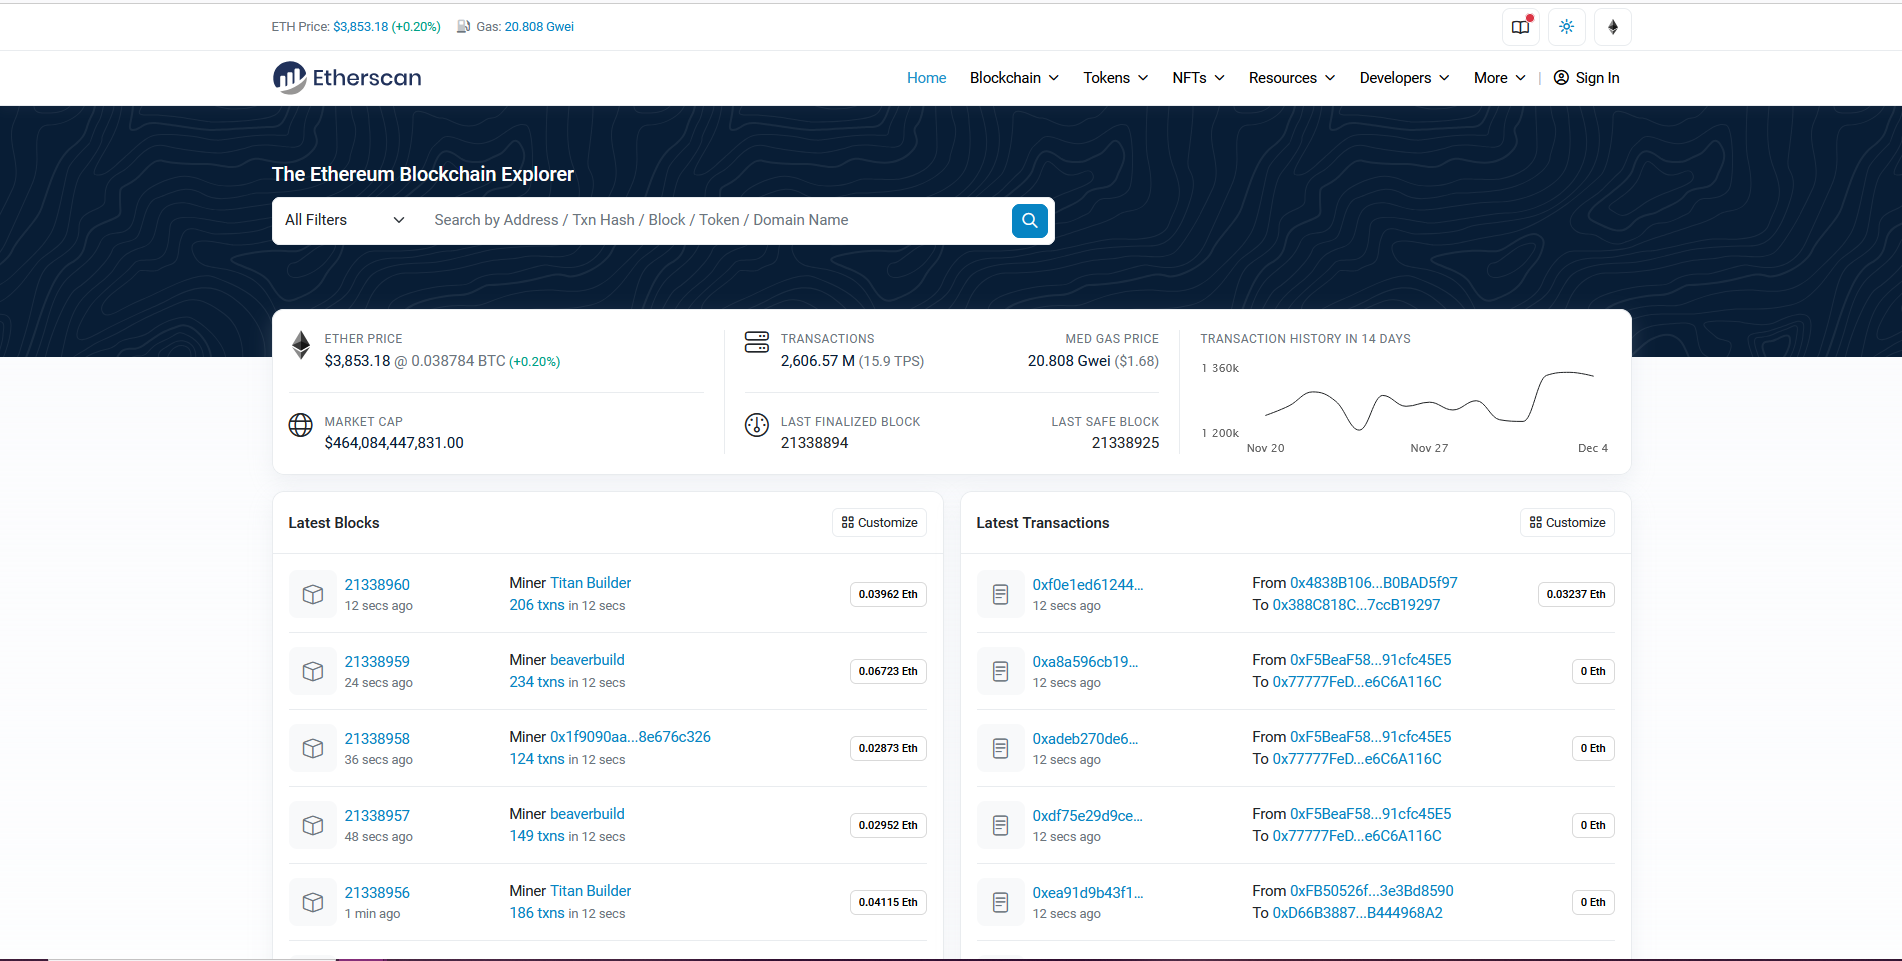
\includegraphics[width=0.8\linewidth]{./obrazy/Etherscan.png}
    \caption{Etherscan}
    \label{fig:Etherscan}
\end{figure}
W odpowiedzi na te braki dobrym pomysłem byłoby stworzenie platformy zapewniającej użytkownikom nie tylko dostęp do wiedzy, ale także pozwalającej na bezpośrednie sprawdzania danych z blockchainów, takich jak aktualne transakcje, stan kont oraz informacje o stanie sieci. Pomysł ten stał się podstawą do zdefiniowania tematu niniejszej pracy.


\section{Cel i zakres pracy}
Celem niniejszej pracy inżynierskiej jest zaprojektowanie i zaimplementowanie platformy internetowej przeznaczonej dla użytkowników kryptowalut i technologii blockchain. Ma ona służyć nie tylko poszerzaniu wiedzy, ale także otworzyć dostęp do funkcji pozwalających na bezpośrednie sprawdzanie danych z różnych sieci blockchain bez potrzeby korzystania ze specjalizowanych narzędzi przypisanych do poszczególnych sieci.

Platforma ma wspierać trzy główne blockchainy: Bitcoin, Ethereum i Solana, pozwalając użytkownikom na wybór interesującej ich sieci oraz uzyskanie dostępu do aktualnych danych na jej temat. W szczególności powinna ułatwić analizę różnic między blockchainami pod względem struktury bloków oraz funkcjonowania kont użytkowników, oferując funkcje do monitorowania i analizowanie bieżących danych. Dokładniej, platforma powinna umożliwiać:
\begin{itemize}
\item \textbf{przeglądanie szczegółowych informacji o wybranych blockchainach}, takich jak dane bloków, transakcji i kont; 
\item \textbf{bezpośrednie sprawdzanie danych z sieci blockchain} poprzez integrację z API, np.\ Alchemy (co pozwoli na weryfikację stanu kont, przeglądanie historii transakcji oraz monitorowanie stanu sieci  w czasie rzeczywistym, np.\ monitorowanie liczby aktywnych węzłów czy bieżącej opłaty transakcyjnej);
\item \textbf{symulację transakcji na blockchainie Solana}, co ułatwi użytkownikom zrozumienie procesu przesyłania środków w rzeczywistej sieci;
\item \textbf{dostęp do przewidywań cen kryptowalut z wykorzystaniem modeli sztucznej inteligencji}, co wyrobić ma dobre nawyki oraz pozwolić na lepsze planowanie inwestycji;
\item \textbf{konwersję walut tradycyjnych na kryptowaluty oraz odwrotnie}, co pozwoli na szybkie obliczenia związane z inwestycjami. 
\end{itemize}

Realizacja projektu wymaga zastosowania zaawansowanych technologii i narzędzi programistycznych, co nadaje pracy charakter inżynierski. Frontend platformy zostanie zbudowany w technologii React, co zapewni dynamiczny i responsywny interfejs użytkownika, umożliwiający łatwe przeglądanie danych oraz wykonywanie operacji. Backend, stworzony przy użyciu frameworka Spring Boot, będzie odpowiedzialny za integrację z zewnętrznymi API oraz przetwarzanie danych blockchainowych w sposób bezpieczny i wydajny. Wdrożenie platformy odbędzie się z wykorzystaniem rozwiązań chmurowych, takich jak Amazon Web Services (AWS), co zapewni elastyczność, skalowalność i niezawodność systemu.

Szczególny nacisk zostanie położony na bezpieczeństwo przetwarzania i przesyłania danych blockchainowych. Platforma będzie wykorzystywać szyfrowanie danych, co zapewni ochronę wrażliwych informacji użytkowników oraz ich transakcji. Dzięki temu użytkownicy będą mogli wykonywać operacje na blockchainie bez obaw o bezpieczeństwo swoich danych.

\section{Układ pracy} W niniejszej pracy omówione zostaną następujące zagadnienia:
W rozdziale drugim zostaną przedstawione: analiza wymagań, architektura systemu, Komponenty systemu, Interakcje między komponentami, Wymagania aplikacji, Przykłady użycia aplikacji, Wymagania niefunkcjonalne
\chapter{Analiza wymagań}
W rozdziale przedstawiono analizę wymagań, od ogólnych założeń po szczegóły dotyczące zarówno planowanych funkcji systemu, jak i aspektów technicznych związanych z implementacją. Opisano też kluczowe funkcje platformy, takie jak przeglądanie danych blockchainowych, zarządzanie kryptowalutami i NFT, symulacje transakcji oraz przewidywanie cen z wykorzystaniem modeli AI. Wyróżnikiem aplikacji jest integracja z zewnętrznymi API blockchainowymi, co umożliwia dynamiczne pobieranie danych w czasie rzeczywistym i oferowanie unikalnych funkcji dla użytkowników.

\section{Założenia ogólne}
Przystępując do realizacji projektu założono, że budowana platforma będzie oferować użytkownikom szeroki wachlarz funkcji, umożliwiając im nie tylko naukę, ale także interakcję z rzeczywistymi danymi blockchainowymi. Zakres tych interakcji opisano w punktach poniżej.
\begin{itemize}
\item \textbf{Wybór konkretnego blockchaina do analiz i operacji:} platforma będzie oferowała możliwość wyboru obsługiwanego blockchaina, czym różnić się będzie od istniejących serwisów, takich jak Etherscan (skoncentrowanego na Ethereum) czy Solscan (dedykowanego Solanie).
\item \textbf{Sprawdzanie danych z blockchainów}: użytkownicy będą mogli przeglądać aktualne informacje o transakcjach, stanie kont i opłatach w wybranych blockchainach. Dzięki integracji z~Alchemy \cite{alchemy_api}, platforma będzie zapewniała bezpośredni dostęp do danych blockchainowych w~czasie rzeczywistym. 
\item \textbf{Symulacja transakcji na blockchainie Solana}: platforma umożliwi użytkownikom przeprowadzenie symulowanych transakcji, co pozwoli na lepsze zrozumienie mechanizmów przesyłania środków bez ryzyka utraty realnych środków. 
\item \textbf{Przewidywanie cen kryptowalut}: użytkownicy będą mogli uzyskać prognozy dotyczące cen kryptowalut dzięki wykorzystaniu modeli sztucznej inteligencji, co pomoże im w podejmowaniu decyzji inwestycyjnych. Model ten będzie analizować dane historyczne i bieżące, generując prognozy, które będą udostępniane użytkownikom w aplikacji.
\item \textbf{Dostęp do materiałów edukacyjnych}: platforma będzie zawierać linki do kursów wideo, artykułów oraz innych materiałów edukacyjnych, które pozwolą użytkownikom poszerzać wiedzę na temat technologii blockchain. 
\item \textbf{Konwersja walut i kryptowalut}: funkcja konwertera ułatwi przeliczenia pomiędzy walutami tradycyjnymi a kryptowalutami, co jest istotne dla inwestorów. 
\end{itemize}
Sposób sposobu dostarczenia tych funkcji wymaga dalszego komentarza:
\begin{itemize}
\item Aplikacja powinna obsługiwać wielu użytkowników, spełniając przy tym wymogi bezpieczeństwa. Dlatego powinna oferować możliwość zarządzania danymi użytkowników, w~tym rejestrację i logowanie za pomocą bezpiecznego mechanizmu autoryzacji opartego na OAuth2 i~tokenach JWT. 
\item Użytkownicy muszą mieć możliwość przeglądania szczegółowych danych blockchainowych, takich jak transakcje, bloki i konta na blockchainach Bitcoin, Ethereum i Solana. System powinien także umożliwiać dynamiczne wyszukiwanie tych danych za pomocą zapytań REST, które frontend przesyła do backendu.
\item Dostęp do bieżących danych o transakcjach i stanie blockchainów będzie możliwy dzięki integracji z ich API. Zwiększy to wartość informacyjną platformy i pozwoli na podejmowanie bardziej świadomych decyzji inwestycyjnych.
\item Aplikacja powinna zapewniać prezentację kategorii kryptowalut, danych historycznych oraz informacji o rynku globalnym, takich jak wskaźnik strachu i chciwości. 
\item Użytkownicy powinni mieć dostęp do danych związanych z NFT, w tym szczegółowych informacji o kolekcjach i tokenach oraz ich statystykach. System musi również umożliwiać realizację operacji blockchainowych, takich jak symulacje transakcji czy airdropy, które są wykonywane za pomocą dedykowanych skryptów Node.js.
\end{itemize}

Pod względem niefunkcjonalnym aplikacja musi być wydajna, obsługując wiele równoczesnych zapytań REST bez znaczącego spadku wydajności. Dynamiczne pobieranie danych blockchainowych z zewnętrznych API, takich jak Etherscan \cite{etherscan_api} czy CoinMarketCap \cite{coinmarketcap_api}, musi odbywać się w czasie rzeczywistym z minimalnym opóźnieniem. System musi być skalowalny.

\subsection{Zarys architektury}\label{subsec:ZarysArchitektury}
Architektura systemu opierać się na modularnym podejściu, z wyraźnym podziałem na frontend i backend, wspierane przez skrypty Node.js i Python oraz bazę danych PostgreSQL. Dzięki konteneryzacji każdy komponent powinien dać się uruchomić w izolowanym środowisku. Interakcje między komponentami odbywać się mają za pomocą protokołu REST, z uwierzytelnieniem opartym na OAuth2 i tokenach JWT.

Zarys architektury budowanego systemu pokazano na rysunku~\ref{fig:ZarysyArchitekturySystemu}.
\begin{figure}[htb] %TO DO: proszę zamiast png wygenerować pdf
    \centering
    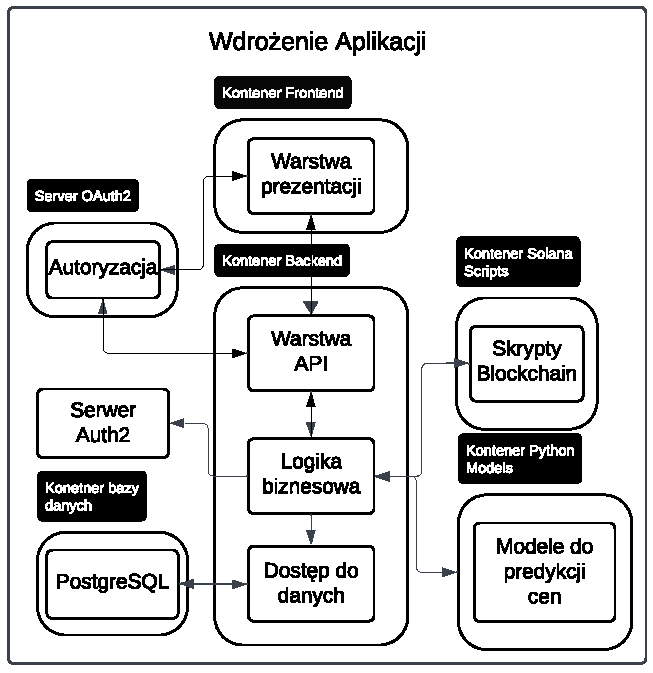
\includegraphics[width=0.7\linewidth]{Diagram.pdf}
    \caption{Zarysy architektury systemu}
    \label{fig:ZarysyArchitekturySystemu}
\end{figure}

Każdy komponent działać ma jako osobny moduł, uruchamiany w odrębnym kontenerze Docker, co zapewnić ma izolację środowisk oraz łatwość wdrażania i utrzymania. Komunikacja między frontendem a~backendem odbywać się ma za pomocą protokołu REST, z odpowiedziami zwracanymi w formacie JSON, w postaci obiektów \texttt{ResponseEntity}, co ułatwi integrację i zapewni spójność przesyłanych danych.

Bezpieczeństwo aplikacji jest priorytetem. Wszystkie dane przesyłane między frontendem a~backendem muszą być zabezpieczone za pomocą szyfrowania HTTPS, a tokeny JWT muszą być przechowywane w sposób bezpieczny w przeglądarce użytkownika. System musi być odporny na ataki oraz zapewniać ochronę przed nieautoryzowanym dostępem.

Backend, pełniący rolę centralnego punktu przetwarzania danych, zostanie zaimplementowany w Spring Boot 3 z użyciem Javy 21. Do zarządzania danymi użytkowników oraz NFT w bazie PostgreSQL wykorzystany zostanie \texttt{CrudRepository} ze Spring Data JPA. Informacje blockchainowe, takie jak transakcje i dane tokenów, będą pobierane w czasie rzeczywistym z~API dostawców, takich jak Etherscan \cite{etherscan_api} i CoinMarketCap \cite{coinmarketcap_api} (zakłada się możliwość zamockowania tych API do celów testowania). Backend dodatkowo wykorzystany zostanie Node.js do realizacji zaawansowanych operacji blockchainowych, w tym symulacji transakcji oraz airdropów.

Frontend, zbudowany w React, działać ma jako aplikacja wielostronicowa MPA (ang.~\emph{Multi-Page Application}). Komunikację z backendem zapewnić ma użycie biblioteki \texttt{axios}. Autoryzacja użytkowników zostanie realizowana za pomocą tokenów JWT przechowywanych w~\texttt{localStorage}, co zapewni bezpieczeństwo sesji oraz ochronę komunikacji między komponentami.

System musi być również łatwy w utrzymaniu. Kod aplikacji musi być zgodny z najlepszymi praktykami programistycznymi. Planowane jest wdrożenie pipeline’u CI/CD do automatyzacji procesu budowy, testowania i wdrażania.

\section{Analiza wymagań}
Na podstawie założeń ogólnych sformułowano wymagania szczegółowe. Zestawiono je poniżej. Stanowią one uzupełnienie do opisanych już założeń ogólnych. 
\subsection{Wymagania dziedzinowe}
Zebrane poniżej wymagania podzielono na grupy w zależności od domeny ich zastosowania. %Poniżej przedstawiono szczegóły każdej z tych grup.

\paragraph{Kategorie i dane rynkowe}
\begin{itemize}
\item \textbf{Category} -- reprezentuje kategorię kryptowalut (np.\ DeFi, NFT), z jej nazwą i opcjonalnym opisem. System powinien umożliwiać wyświetlanie kategorii kryptowalut.
\item \textbf{Cryptocurrency} -- reprezentuje kryptowalutę, jej nazwę, symbol i dane rynkowe.
\item \textbf{HistoricalData} -- reprezentuje dane historyczne kryptowalut (cena, wolumen, kapitalizacja). System powinien umożliwiać przechowywanie danych historycznych i zapytanie o dane w~określonym dniu w przeszłości.
\item \textbf{FearAndGreed} -- reprezentuje wskaźnik strachu i chciwości na rynku kryptowalut. System powinien umożliwiać pobieranie bieżących.
\end{itemize}

\paragraph{Dane NFT}
\begin{itemize}
\item \textbf{Collection} -- reprezentuje kolekcję NFT, np.\ Bored Ape Yacht Club. Przechowuje nazwę, opis, liczbę tokenów w kolekcji oraz właścicieli. Powiązana z tokenami NFT.
\item \textbf{CollectionStats} -- przechowuje dane statystyczne kolekcji NFT, np. średnia cena, wolumen obrotu. Umożliwia aktualizację danych na podstawie transakcji.
\item \textbf{NFT} -- reprezentuje token NFT, w tym metadane, właściciela i historię transakcji.
\item \textbf{NFTOwner} -- przechowuje dane właścicieli NFT, np.\ ID użytkownika i adres portfela. Obsługuje powiązania między właścicielami a tokenami.
\item \textbf{NFTRarity} -- reprezentuje rzadkość tokenu NFT w skali procentowej.
\item \textbf{NFTTrait} -- przechowuje cechy tokenów NFT, np.\ tło. Obsługuje mapowanie cech na tokeny.
\end{itemize}

\paragraph{Dane blockchainowe Bitcoin}
\begin{itemize}
\item \textbf{BitcoinAccount} -- reprezentuje konto w sieci Bitcoin. Umożliwia zmapowanie surowych danych, przekształcając je w strukturę obiektową.
\item \textbf{BitcoinBlock} -- reprezentuje blok w sieci Bitcoin. Umożliwia zmapowanie surowych danych, przekształcając je w strukturę obiektową.
\item \textbf{BitcoinTransaction} -- reprezentuje transakcję w sieci Bitcoin. Umożliwia zmapowanie surowych danych, przekształcając je w strukturę obiektową.
\end{itemize}

\noindent Analogicznie będzie dla folderów Etherum oraz Solana.\\[-20pt]
\paragraph{Dodatkowe dane blockchainowe Ethereum}
\begin{itemize}
\item \textbf{Contract} -- reprezentuje inteligentny kontrakt Ethereum. Przechowuje kod, adres i ABI. Umożliwia interakcję z kontraktami i odczyt/zapis danych na blockchainie.
\end{itemize}

\paragraph{Dodatkowe dane blockchainowe Solana}
\begin{itemize}
\item \textbf{Epoch} -- reprezentuje epokę w sieci Solana, przechowuje liczbę slotów i czas trwania. Obsługuje dynamiczne aktualizacje danych w zależności od stanu sieci.
\item \textbf{SolanaClusterNode} -- reprezentuje węzeł Solana, zawiera adres IP, status i typ roli (np. walidator). Umożliwia monitorowanie stanu węzłów klastra.
\item \textbf{SplToken} -- reprezentuje token SPL, przechowuje symbol, nazwę, liczbę dziesiętnych miejsc i adres kontraktu. Obsługuje zapytania o szczegóły tokenu i jego emisję.
\end{itemize}

\subsection{Przypadki użycia aplikacji}
Aplikacja powinna umożliwiać realizację różnych scenariuszy użytkowania, stosownie do potrzeb użytkowników zainteresowanych blockchainami, kryptowalutami i NFT. Poniżej przedstawiono główne przypadki jej potencjalnego użycia.

\paragraph{Przeglądanie danych blockchainowych}
Użytkownik loguje się do aplikacji, a następnie może przeglądać szczegółowe dane blockchainowe dotyczące Bitcoin, Ethereum i Solana. Na przykład może wyszukiwać adresy blockchainowe, aby uzyskać historię transakcji, saldo lub dane o blokach, takie jak wysokość i czas utworzenia. Dane są pobierane w czasie rzeczywistym z~zewnętrznych API, co zapewnia aktualność informacji.

\paragraph{Analiza kryptowalut i danych rynkowych}
Użytkownik może przeglądać kategorie kryptowalut, ich dane historyczne oraz informacje o rynku globalnym, ze wskaźnikami strachu i~chciwości. Historia cen kryptowalut może objąć 2 ostatnie lata, zaś dane dotyczyć mogą wolumenu obrotu dla wybranej kategorii, co może pomóc w podejmowanie decyzji inwestycyjnych.

\paragraph{Zarządzanie kolekcjami NFT}
Aplikacja pozwala przeglądać szczegóły dotyczące kolekcji NFT. Użytkownik może również wyszukiwać pojedyncze tokeny i sprawdzać ich metadane oraz historię transakcji. To przydatne dla kolekcjonerów i inwestorów NFT.

\paragraph{Symulacje transakcji blockchainowych}
Za pomocą skryptów Node.js użytkownik może symulować transakcje blockchainowe takie jak przesyłanie tokenów lub wykonywanie airdropów. Po wykonaniu operacji użytkownik dostanie informację na temat rezultatów operacji.

\paragraph{Wykorzystanie AI do przewidywania cen kryptowalut}
Model AI zintegrowany z aplikacją umożliwi prognozowanie cen kryptowalut. Użytkownik będzie wybierał datę a następnie będzie mógł zobaczyć przewidywaną cenę Bitcoina, Etheru i Sol. Wyniki są prezentowane w formie pojedyńczej wartości, co wspiera podejmowanie decyzji inwestycyjnych.

\paragraph{Dynamiczne przetwarzanie danych blockchainowych}
Aplikacja pozwala uzyskać dane blockchainowe w czasie rzeczywistym dzięki dynamicznym połączeniom z API dostawców. Użytkownik może np. przeglądać najnowsze transakcje w sieci Solana lub analizować szczegóły tokenów ERC-20 na Ethereum. Funkcjonalność ta jest kluczowa dla osób potrzebujących aktualnych danych.

\subsection{Wymagania niefunkcjonalne}
Wymagania niefunkcjonalne aplikacji koncentrują się na wydajności, skalowalności, bezpieczeństwie oraz łatwości utrzymania. Planowane wdrożenie w chmurze AWS z wykorzystaniem Elastic Load Balancer (ELB) pozwolić ma na dynamiczne zarządzanie zasobami i równoważenie obciążenia. Dodatkowo, zastosowanie pipeline’u CI/CD usprawni procesy związane z utrzymaniem i rozwojem systemu, zapewniając jego długoterminową stabilność. Wymagania te uszczegółowiono poniżej.

\paragraph{Wydajność}
Backend musi obsługiwać co najmniej 100 równoczesnych zapytań REST bez znaczącego spadku wydajności. Dynamiczne pobieranie danych blockchainowych z zewnętrznych API musi odbywać się w czasie rzeczywistym z minimalnym opóźnieniem, aby zapewnić użytkownikom aktualne informacje.

\paragraph{Skalowalność}
System musi być skalowalny i dostosowany do zwiększającej się liczby użytkowników. Planowane wdrożenie w chmurze AWS z wykorzystaniem Elastic Load Balancer (ELB) umożliwi równoważenie obciążenia oraz dynamiczne zarządzanie zasobami.

\paragraph{Bezpieczeństwo}
Wszystkie dane przesyłane między frontendem a backendem muszą być zabezpieczone szyfrowaniem HTTPS. Tokeny JWT muszą być bezpiecznie przechowywane w~\texttt{localStorage} i weryfikowane przez backend przy każdym zapytaniu. System musi być odporny na ataki CSRF i XSS, a dane użytkowników muszą być chronione przed nieautoryzowanym dostępem.

\paragraph{Niezawodność}
Aplikacja musi zapewniać 99,9\% dostępności, co zostanie osiągnięte dzięki konteneryzacji oraz planowanemu wdrożeniu na AWS. Mechanizmy monitorowania i powiadamiania o błędach lub awariach muszą zapewnić szybką reakcję na problemy.

\paragraph{Elastyczność}
Architektura aplikacji musi umożliwiać łatwe dodawanie nowych funkcjonalności, takich jak obsługa kolejnych blockchainów czy wdrażanie modeli analitycznych AI. Modularna budowa, w której każdy komponent działa jako niezależny kontener Docker, wspiera tę elastyczność.

\paragraph{Łatwość utrzymania}
Kod aplikacji musi być zgodny z najlepszymi praktykami, w tym zasadami SOLID i wzorcami projektowymi, co zapewni jego łatwą rozbudowę i utrzymanie. Planowane wdrożenie pipeline'u CI/CD usprawni procesy budowy, testowania i wdrażania.

\paragraph{Zgodność technologiczna}
Aplikacja musi działać w środowisku obsługującym Dockera. Backend opiera się na Javie 21 i Spring Boot 3, a frontend został zaimplementowany w React, co zapewnia kompatybilność z nowoczesnymi przeglądarkami, takimi jak Chrome, Firefox i Safari.\\


Podsumowując, aplikacja ma być wszechstronnym narzędziem, które dzięki modularnej architekturze i zaawansowanym funkcjom sprosta wymaganiom zarówno inwestorów, jak i entuzjastów blockchainów. System oferować ma wysoką elastyczność i bezpieczeństwo, co uczyni go odpowiednim rozwiązaniem dla dynamicznie zmieniającego się rynku kryptowalut i technologii blockchain.


\chapter{Implementacja}
W niniejszym rozdziale opisano proces, którego celem było zaimplementowanie platformy spełniającej postawione wcześniej wymagania funkcjonalne oraz niefunkcjonalne. 
W procesie tym wystąpiły wszystkie kluczowe kroki, począwszy od konfiguracji środowiska, przez rozwój aplikacji backendowej i frontendowej, aż po integrację z systemami zewnętrznymi oraz konfigurację kontenerów Dockerowych. Lektura tego rozdziału powinna pozwolić na zapoznanie się ze szczegółami implementacji, uwagami dotyczącymi użytych technologii, narzędzi oraz metodami, które umożliwiły realizację tak założonego projektu.

W rozdziale omówione zostaną aspekty techniczne implementacji, w tym struktura repozytoriów kodu, konfiguracja środowiska developerskiego, użyte frameworki i biblioteki, oraz zagadnienia związane z budową i wdrożenia aplikacji. Zaznaczono w nim główne decyzje architektoniczne, które wpłynęły na projektowanie aplikacji oraz integrację z systemami zewnętrznymi, w tym bazami danych, serwerami aplikacji oraz kontenerami Dockerowymi.

Podczas implementacji, szczególną uwagę poświęcono skalowalności aplikacji, zapewnieniu bezpieczeństwa danych oraz optymalizacji wydajności. Każdy z komponentów systemu – zarówno backend jak i frontend – został zaprojektowany w sposób umożliwiający łatwą rozbudowę oraz integrację z dodatkowymi usługami w przyszłości.


\section{Podział logiczny}
\subsection{Komponenty systemu}
Zgodnie z założeniami co do architektury, podczas implementacji stworzono główne moduły systemu: frontend oraz backend (patrz podrozdział~\ref{subsec:ZarysArchitektury}).\\[-10pt]

\noindent \textbf{Frontend} -- %zbudowany w React jako aplikacja wielostronicowa (MPA), % to już było w założeniach ogólnych
odpowiada za prezentację danych i interakcję z użytkownikami. Podzielono go na moduły odpowiadające różnym domenom funkcjonalnym. Moduł blockchain prezentuje dane związane z blockchainami Bitcoin, Ethereum i Solana, w tym szczegóły transakcji, bloków oraz kont. Ten moduł zawiera podkomponenty obsługujące wyszukiwanie oraz wyświetlanie szczegółowych informacji. Moduł kryptowalut zarządza kategoriami kryptowalut, danymi historycznymi, rynkiem globalnym oraz rankingami. Dodatkowo frontend oferuje widoki użytkownika, takie jak logowanie, rejestracja oraz strona główna. Komunikacja z backendem odbywa się za pomocą biblioteki axios, z uwierzytelnianiem opartym na tokenach JWT przechowywanych w \texttt{localStorage}.\\[-10pt]

\noindent \textbf{Backend} -- %zaimplementowany w Spring Boot 3 przy użyciu Javy 21 % to już było w założeniach ogólnych
jest centralnym komponentem systemu. Integruje funkcje związane z logiką biznesową, bazą danych oraz zewnętrznymi dostawcami informacji. Backend udostępnia API REST dla frontendu i obsługuje kilka kluczowych domen, takich jak kryptowaluty, NFT oraz zasoby zewnętrzne. Moduł kryptowalut oferuje funkcje zarządzania kategoriami, danymi historycznymi oraz danymi rynkowymi. Moduł NFT zarządza tokenami, kolekcjami oraz ich statystykami. Backend również integruje dane blockchainowe, takie jak transakcje i bloki, które są dynamicznie pobierane z zewnętrznych API, takich jak Etherscan czy CoinMarketCap. Ponadto backend wywołuje dedykowane skrypty w Node.js w celu realizacji zaawansowanych operacji blockchainowych, takich jak symulacje transakcji i airdropy oraz skrypt w kontenerze Pythonowym, tak aby uzyskać dane o cenie kryptowalut na dany dzień.

Część backendu odpowiada również za bezpieczeństwo, realizowane poprzez mechanizm OAuth2 i tokeny JWT. Tokeny te są wykorzystywane do uwierzytelniania użytkowników oraz zabezpieczania komunikacji między frontendem a backendem. W backendzie baza danych PostgreSQL przechowuje trwałe dane, takie jak użytkownicy, dane NFT oraz kryptowaluty, podczas gdy dane blockchainowe są dynamicznie pobierane i nie są przechowywane.\\[-10pt]

\noindent Ponadto elementami systemu są również różne skrypty. \\[-10pt]

\noindent \textbf{Skrypty Node.js} -- stanowią osobny komponent systemu, uruchamiany w dedykowanym kontenerze Docker. Skrypty te obsługują operacje blockchainowe, takie jak symulacje transakcji, tworzenie nowych kont oraz airdropy tokenów. Współpracują one z backendem, zapewniając wsparcie dla bardziej zaawansowanych funkcjonalności systemu.\\[-10pt]

\noindent \textbf{Skrypt pythonowy} -- stanowi osobny komponent systemu, uruchamiany w dedykowanym kontenerze Docker. Skrypt obsługuje zapytania o przewidywaną wartość kryptowalut na dany dzień. Współpracuje on z backendem zapewniajać dodatkową funkcjonalność.\\[-10pt]

System jest w pełni konteneryzowany, co oznacza, że każdy z jego komponentów — frontend, backend, baza danych, Node.js i ModelContainer -- działają w odrębnych kontenerach Docker. Taka architektura zapewnia izolację środowisk, łatwość wdrażania i możliwość niezależnego skalowania komponentów. W przyszłości system zostanie wdrożony w chmurze AWS z wykorzystaniem Elastic Load Balancer (ELB), co pozwoli na równoważenie obciążenia i zwiększenie wydajności oraz skalowalności.

\subsection{Interakcje między komponentami}
Interakcja między komponentami systemu zaprojektowano korzystając ze standardowych mechanizmów komunikacji, które zapewniają efektywność, bezpieczeństwo i elastyczność działania. System składa się z pięciu głównych komponentów: frontendu, backendu, skryptów Node.js, skryptu w ModelContainer oraz bazy danych PostgreSQL. Każdy z tych komponentów pełni odrębną rolę w architekturze i współpracuje z innymi poprzez jasno zdefiniowane interfejsy.

Frontend pełni rolę warstwy prezentacji. Użytkownicy wchodzą w interakcje z aplikacją korzystając z tego komponentu. Umożliwia on przeglądanie danych blockchainowych, zarządzanie NFT oraz dostęp do funkcji związanych z kryptowalutami. Frontend komunikuje się z backendem za pomocą protokołu REST, korzystając z biblioteki axios. Żądania wysyłane przez frontend zawierają tokeny JWT w nagłówkach, co pozwala na autoryzację użytkowników oraz zapewnia bezpieczeństwo przesyłanych danych. Backend przetwarza żądania, odwołuje się do bazy danych lub zewnętrznych API i zwraca odpowiedzi w formacie JSON.

Komunikacja między frontendem a backendem jest synchroniczna i odbywa się za pomocą REST API. Backend udostępnia RESTful API, które umożliwia frontendowi tworzenie, pobieranie, aktualizowanie danych. Frontend, korzystając z React, wysyła żądania HTTP do backendu za pomocą axios i renderuje odpowiednie dane na interfejsie użytkownika.

Backend działa również jako pośrednik między frontendem a zewnętrznymi dostawcami informacji blockchainowych, takimi jak Etherscan, CoinMarketCap czy Solana RPC, co pozwala na dynamiczne pobieranie danych transakcji, bloków i kont w czasie rzeczywistym. W przypadku bardziej zaawansowanych operacji blockchainowych lub przewidzenia cen, backend wywołuje odpowiednie skrypty. % Dedykować można komuś książkę

Skrypty Node.js działają w osobnym kontenerze i pełnią rolę wspierającą backend w realizacji specyficznych operacji blockchainowych. Skrypty te są wywoływane przez backend za pomocą mechanizmów interfejsowych i umożliwiają wykonywanie działań takich jak generowanie nowych transakcji, symulacje przepływu środków czy zarządzanie airdropami tokenów. Skrypty te operują na danych dynamicznych, które są bezpośrednio pobierane z blockchaina, co eliminuje potrzebę ich zapisywania w bazie danych.

Skrypt pythonowy działa w osobnym kontenerze i pełni rolę wspierającą backend w realizacji przewidywania cen kryptowalut. Skrypt ten jest wykonywany przez backend za pomocą wysłania odpowiedniego żadania na kontener ModelContainer, gdzie serwer odbierze zapytanie i wykona operację przewidzenia ceny. Dane te są następnie zwracane do kontenera backend, tak aby ten mógł je przesłać na frontend.

Baza danych PostgreSQL, jak już wspomniano, przechowuje dane trwałe, takie jak informacje o użytkownikach, kategoriach kryptowalut, danych historycznych oraz NFT. Backend komunikuje się z bazą danych za pomocą warstwy repozytoriów opartej na interfejsach CrudRepository. Gdy użytkownik żąda danych dostępnych w bazie, backend odczytuje je i przekształca w odpowiedzi API, które następnie są przesyłane do frontendu. W przypadku danych blockchainowych, które są dynamiczne, backend bezpośrednio pobiera je z zewnętrznych API, bez konieczności korzystania z bazy danych.

Podsumowując, interakcja między komponentami opiera się na wyraźnym podziale ról i odpowiedzialności. Frontend obsługuje interfejs użytkownika i komunikuje się z backendem poprzez REST API. Backend pełni funkcję centralnego punktu przetwarzania, współpracując zarówno z bazą danych PostgreSQL, jak i z zewnętrznymi dostawcami danych blockchainowych. Skrypty Node.js oraz Python wspierają backend w realizacji specyficznych operacji blockchainowych, a baza danych zapewnia trwałe przechowywanie kluczowych informacji. Wszystkie komponenty współpracują w sposób zintegrowany, zapewniając elastyczność, wydajność i bezpieczeństwo działania systemu.

\section{Podział fizyczny}
Podział logiczny aplikacji przełożył się na jej podział fizyczny i organizację źródeł kodu. Dzięki takiemu podejściu struktura aplikacji stała się czytelna i modularna. Wpłynęło to na łatwość rozbudowy i modyfikacji poszczególnych komponentów. 

Zarówno backend, jak i frontend podzielono na funkcje, co skutkowało lepszą organizację kodu oraz łatwiejszym testowaniem. Integrację frontendu z backendem zrealizowano przy pomocy API. Poniżej przedstawiono szczegółowy opis tych dwóch głównych części aplikacji.

\subsection{Backend}
Backend aplikacji jest napisany w języku Java z wykorzystaniem frameworku Spring Boot. Struktura kodu backendowego jest zgodna z najlepszymi praktykami w zakresie organizacji projektów opartych na tym frameworku. Kluczowe elementy struktury backendu to:
\begin{itemize}
    \item \texttt{src/main/java}: Główna część aplikacji, zawierająca logikę biznesową i kontrolery.
    \item \texttt{src/main/resources}: Pliki konfiguracyjne, w tym \texttt{application.properties}, które służą do konfiguracji bazy danych i innych usług.
    \item \texttt{src/test/java}: Testy jednostkowe oraz integracyjne, zapewniające poprawność działania aplikacji.
    \item \texttt{pom.xml}: Plik konfiguracyjny Maven, który zarządza zależnościami aplikacji.
    \item \texttt{Dockerfile}: Konfiguracja dla Docker, umożliwiająca tworzenie kontenerów dla aplikacji backendowej.
\end{itemize}

\noindent Backend jest podzielony na różne warstwy:
\begin{itemize}
    \item \textbf{Controller}: Warstwa odpowiedzialna za odbiór żądań HTTP i przekazywanie ich do odpowiednich usług.
    \item \textbf{Service}: Warstwa logiki biznesowej, która przetwarza dane i wykonuje operacje na modelach.
    \item \textbf{Repository}: Warstwa odpowiedzialna za komunikację z bazą danych przy użyciu JPA (Java Persistence API).
\end{itemize}
W backendzie każda funkcjonalność została wydzielona do oddzielnych metod w odpowiednich klasach. Przykłady funkcji backendowych:
\begin{itemize}
    \item \texttt{registerUser}: Funkcja tworząca nowego użytkownika w bazie danych.
    \item \texttt{createSolanaAccount}: Funkcja tworząca konto na Solana devnet.
    \item \texttt{getERC20TokenTransfers}: Funkcja pobierająca wszystkie transfery tokenów ERC-20 związane z podanym adresem Ethereum w określonym zakresie bloków (od startBlock do endBlock). Funkcja zwraca listę transakcji w postaci obiektów \texttt{EthereumTransactionDto}.
		\item \texttt{predictPrices}: Funkcja zwracająca przewidywane ceny na dany dzień dla Bitcoina, Etheru i Sol.
\end{itemize}


\subsection{Frontend}
Frontend stworzono z użyciem React -- popularnego frameworku JavaScript, stosowanego do tworzenie dynamicznych interfejsów użytkownika. Struktura kodu frontendowego obejmuje:
\begin{itemize}
    \item \texttt{src/}: Główna część aplikacji frontendowej, zawierająca komponenty, funkcje oraz logikę.
    \item \texttt{public/}: Pliki statyczne, takie jak HTML, obrazy, czcionki itp.
    \item \texttt{package.json}: Plik konfiguracyjny npm, zarządzający zależnościami aplikacji.
    \item \texttt{Dockerfile.dev}: Plik konfiguracyjny Docker dla środowiska deweloperskiego.
\end{itemize}
Frontend jest podzielony na następujące elementy:
\begin{itemize}
    \item \textbf{Komponenty}: Aplikacja frontendowa jest zbudowana w oparciu o komponenty React, które reprezentują poszczególne elementy interfejsu użytkownika.
    \item \textbf{Logika aplikacji}: Funkcje obsługujące interakcje użytkownika, komunikację z backendem oraz zarządzanie stanem aplikacji.
    \item \textbf{Routing}: Aplikacja frontendowa wykorzystuje React Router do zarządzania nawigacją pomiędzy różnymi widokami aplikacji.
\end{itemize}


Kod frontendu podzielono na mniejsze fragmenty, stosownie do implementowanych funkcji:
\begin{itemize}
    \item \texttt{fetchData} -- funkcja do pobierania danych z API backendu.
    \item \texttt{handleSubmit} --funkcja obsługująca zdarzenie wysyłania formularza, aby dostać dane ze specyficznego dnia.
    \item \texttt{navigateToDetails} -- funkcja nawigująca do strony szczegółów na podstawie wprowadzonego adresu.
\end{itemize}




\section{Konteneryzacja}
Aplikacja została zaprojektowana z wykorzystaniem kontenerów Docker, które umożliwiają izolację poszczególnych komponentów systemu oraz łatwą konfigurację środowiska developerskiego i produkcyjnego. Kontenery są połączone ze sobą w sieci Docker, co umożliwia ich wzajemną komunikację. Poniżej przedstawiono szczegółowy opis zależności między kontenerami w systemie oraz roli, jaką pełni każdy z nich.

\subsection{Architektura kontenerów}
W systemie zostały zaimplementowane następujące kontenery:
\begin{itemize}
    \item \textbf{Kontener backendowy} – zawiera aplikację backendową, która realizuje logikę biznesową, obsługę żądań HTTP, komunikację z bazą danych oraz integrację z zewnętrznymi API.
    \item \textbf{Kontener frontendowy} – zawiera aplikację frontendową napisaną w React, która komunikuje się z backendem, wyświetlając dane użytkownikowi i obsługując interakcje z interfejsem.
    \item \textbf{Kontener Node.js} – zawiera środowisko Node.js, które uruchamia skrypty do komunikacji z blockchainem Solany. Kontener ten jest odpowiedzialny za tworzenie konta na blockchainie devnet Solany, symulowanie transakcji oraz wykonywanie operacji airdrop.
    \item \textbf{Kontener bazy danych PostgreSQL} – przechowuje dane aplikacji, w tym dane użytkowników, transakcje, informacje o przedmiotach do wynajmu itp. Komunikacja z bazą danych odbywa się za pośrednictwem warstwy repozytoriów w aplikacji backendowej.
		\item \textbf{Kontener ModelContainer} - zawiera skrypt napisany w języku Python, który umożliwia dostanie przewidzianej ceny dla danych kryptowalut na dany dzień.
    \item \textbf{Kontener pgAdmin} – jest narzędziem do zarządzania bazą danych PostgreSQL, umożliwiającym administrację i monitorowanie bazy danych za pomocą interfejsu graficznego.
\end{itemize}

\subsection{Zależności między kontenerami}
Kontenery w systemie są ze sobą powiązane, umożliwiając ich współpracę. Każdy kontener komunikuje się z innymi, zapewniając sprawne funkcjonowanie aplikacji jako całości. Wszystkie kontenery znajdują się na jednej sieci, co umożliwia im wymianę danych i współpracę. 

Kontener frontendowy współpracuje z backendem, który realizuje logikę aplikacji i komunikuje się z bazą danych PostgreSQL. Kontener Node.js odgrywa kluczową rolę w integracji aplikacji z blockchainem Solany, wykonując skrypty do pobierania i przetwarzania danych. Kontener  ModelContainer odpowiedzialny jest za zarządzanie modelami i przewidywanie cen. Dzięki zastosowaniu Docker Compose możliwe jest łatwe zarządzanie tymi kontenerami, ich konfiguracja oraz zapewnienie ich współpracy w ramach jednej sieci. Takie podejście pozwala na łatwą skalowalność aplikacji i rozdzielenie odpowiedzialności między poszczególne komponenty. Poniżej opisano zależności między kontenerami:
\begin{itemize}
    \item \textbf{Kontener frontendowy i backendowy}: Kontener frontendowy, odpowiedzialny za interfejs użytkownika, wysyła żądania HTTP do kontenera backendowego. Aplikacja frontendowa, napisana w React, korzysta z API udostępnionego przez aplikację backendową za pomocą axios do pobierania i wysyłania danych. Komunikacja odbywa się przez porty udostępnione w konfiguracji Docker Compose.
    \item \textbf{Kontener backendowy i baza danych PostgreSQL}: Aplikacja backendowa komunikuje się z bazą danych PostgreSQL w celu przechowywania i pobierania danych. Backend korzysta z JPA (Java Persistence API) do wykonywania operacji CRUD na bazie danych.
    \item \textbf{Kontener backendowy i kontener Node.js}: Kontener Node.js pełni rolę interfejsu między aplikacją backendową a blockchainem Solany w kontekście wykonywania operacji na blockchainie, a nie pobieraniu danych z niego. Backend wysyła zapytania do kontenera Node.js w celu wykonania skryptów Solany, które mogą tworzyć konto, symulować transakcję oraz wykonywać operację airdrop. Kontener Node.js uruchamia odpowiednie skrypty do interakcji z blockchainem, wykorzystując bibliotekę @solana/web3.js.
		\item \textbf{Kontener backendowy i kontener ModelContainer}: Aplikacja backendowa wysyła zapytanie na kontener ModelContainer, tak aby uzyskać dane dotyczące przewidzianych cen. 
    \item \textbf{Kontener Node.js i blockchain Solany}: Kontener Node.js, uruchamiający skrypty Solany, komunikuje się z siecią blockchain Solany poprzez RPC endpointy. Skrypty w kontenerze Node.js są odpowiedzialne za tworzenie konta, symulowanie transakcji oraz wykonywanie operacji airdrop. Wyniki tych skryptów są następnie odbierane przez klasę serwisą, i zwracane do kontrolera, który wysyłaja je na frontend.
    \item \textbf{Kontener pgAdmin i baza danych PostgreSQL}: Kontener pgAdmin umożliwia zarządzanie bazą danych PostgreSQL poprzez interfejs graficzny. Administratorzy mogą monitorować, modyfikować oraz zarządzać strukturą bazy danych, korzystając z pgAdmin, który łączy się z kontenerem bazy danych PostgreSQL.
\end{itemize}

\section{Budowa aplikacji za pomocą Maven i Docker}
Podczas budowy aplikacji wykorzystano narzędzia Maven i Docker. Pozwoliło to na efektywne zarządzanie  zależnościami projektowymi oraz środowiskiem uruchomieniowym. Maven posłużył jako system zarządzania projektem, wspierający kompilację, testowanie i pakowanie aplikacji. Dodatkowo pomógł on w zarządzaniu pakietami potrzebnymi do działania aplikacji. Docker umożliwił konteneryzację aplikacji, zapewniając spójność środowiska uruchomieniowego niezależnie od platformy. Obrazy kontenerów budowano w oparciu o pliki \texttt{Dockerfile}, zawierające definicje zależności oraz konfiguracje potrzebne do uruchomienia aplikacji. 

Aby zbudować obraz dla aplikacji backendowej należy wykonać:
\begin{lstlisting}[basicstyle=\footnotesize\ttfamily]
docker build -t backend_image .
\end{lstlisting}

Aplikacja frontendowa oparta na React ma swój własny plik \texttt{Dockerfile}, który zawiera instrukcje do budowy aplikacji. Aby go zbudować należy wpisać komendę:
\begin{lstlisting}[basicstyle=\footnotesize\ttfamily]
docker build -t frontend_image .
\end{lstlisting}

%Analogicznie należy postąpić dla obrazu solana_scripts\_image i model\_server

Po zbudowaniu obrazów kontenery mogą zostać uruchomione przy pomocy \texttt{docker compose up}. Poniżej przykład pliku \texttt{docker-compose.yml}, który definiuje kontener frontend:
\begin{lstlisting}[basicstyle=\footnotesize\ttfamily]
  frontend_app:
    image: frontend_image
    container_name: frontend_app
    volumes:
      - ./frontend:/usr/app
    ports:
      - "3000:3000"
    command: ["npm", "start"]
    networks:
      - my_network
\end{lstlisting}

\subsection{Konfiguracja narzędzi} 

\subsubsection{Zależności i wtyczki Maven}
W projekcie wykorzystano pluginy Maven automatyzujące budowę aplikacji. Były to głównie pluginy: \texttt{maven-clean-plugin}, \texttt{maven-compiler-plugin}, \texttt{maven-jar-plugin}, \texttt{maven-surefire-plugin}, oraz \texttt{spring-boot-maven-plugin}.
Jeśli chodzi o zależności, projekt korzysta z kluczowych bibliotek jak \texttt{spring-boot-starter-web}, \texttt{spring-boot-starter-data-jpa}, \texttt{postgresql}, \texttt{spring-security}, \texttt{lombok}, i \texttt{mysql-connector-java}.

%%%%%%%%%%%%%%%%%%%%%%%%%%%%%%%%%%%
\subsubsection{Struktura pliku Dockerfile dla aplikacji backendowej}

Plik \texttt{Dockerfile} zawiera instrukcje, które definiują sposób budowy obrazu Docker dla aplikacji. Poniżej opisano strukturę pliku \texttt{Dockerfile}, z uwzględnieniem najważniejszych instrukcji, bazujących na dwufazowej budowie obrazu.\\[-10pt]

\noindent \textbf{Podstawowy obraz~~}
Plik \texttt{Dockerfile} pozwala zdefiniować obraz bazowy. W pracy skorzystano z dwóch obrazów: do budowy aplikacji w pierwszej fazie oraz do jej uruchomienia w drugiej fazie. Do budowy użyto obrazu \texttt{amazoncorretto:21-alpine}, który zawiera OpenJDK 21, zaś do uruchomienia obraz \texttt{ubuntu:24.04}. Obraz bazowy definiuje się komendą \texttt{FROM}:
\begin{lstlisting}[basicstyle=\footnotesize\ttfamily]
FROM amazoncorretto:21-alpine AS build
\end{lstlisting}

\noindent \textbf{Instalowanie Maven i kompilacja aplikacji~~}
W pierwszej fazie instalowany jest Maven za pomocą komendy \texttt{RUN apk add --no-cache maven}, aby pobrać zależności aplikacji i ją skompilować. następnie kopiowany jest plik \texttt{pom.xml} oraz kod źródłowy aplikacji do obrazu. Następnie uruchamiany jest Maven do pobrania zależności i zbudowania aplikacji:
\begin{lstlisting}[basicstyle=\footnotesize\ttfamily]
RUN apk add --no-cache maven
COPY pom.xml .
RUN mvn dependency:go-offline
COPY src ./src
RUN mvn package -DskipTests
\end{lstlisting}

\noindent \textbf{Tworzenie obrazu do uruchomienia aplikacji~~}
W drugiej fazie instalowane są wszystkie niezbędne zależności do uruchomienia aplikacji. Używany jest obraz \texttt{ubuntu:24.04}, aby zainstalować wymagane pakiety, takie jak \texttt{openjdk-21-jdk}, \texttt{openssl}, \texttt{docker.io} oraz \texttt{curl}:
\begin{lstlisting}[basicstyle=\footnotesize\ttfamily]
FROM ubuntu:24.04
RUN apt-get update && \
    apt-get install -y --no-install-recommends \
    curl \
    ca-certificates \
    openjdk-21-jdk \
    docker.io \
    openssl && \
    apt-get clean && \
    rm -rf /var/lib/apt/lists/*
\end{lstlisting}

\noindent \textbf{Kopiowanie pliku JAR i generowanie kluczy RSA~~}
Po zainstalowaniu zależności, kopiowany jest plik JAR do obrazu i generowane są klucze RSA, które będą używane przez aplikację do obsługi autoryzacji OAuth2. Wygenerowane klucze publiczny i prywatny są następnie konwertowane do formatu PKCS\#8.
\begin{lstlisting}[basicstyle=\footnotesize\ttfamily]
COPY --from=build /app/target/*.jar app.jar
RUN openssl genrsa -out keypair.pem 2048
RUN openssl rsa -in keypair.pem -pubout -out publicKey.pem
RUN openssl pkcs8 -topk8 -inform PEM -outform PEM -nocrypt -in keypair.pem -out privateKey.pem
\end{lstlisting}

\noindent \textbf{Uruchamianie aplikacji}
Po zbudowaniu obrazu, kontener jest uruchamiany. Użyta zostaje komenda \texttt{ENTRYPOINT}, aby określić, jak uruchomić aplikację. W tym przypadku aplikacja jest uruchamiana za pomocą komendy \texttt{java -jar} z odpowiednimi parametrami konfiguracyjnymi dla serwera i kluczy publicznego oraz prywatnego.
\begin{lstlisting}[basicstyle=\footnotesize\ttfamily]
ENTRYPOINT ["java", "-jar", "app.jar", \
    "--server.port=8080", \
    "--spring.security.oauth2.resourceserver.jwt.public-key-location=classpath:publicKey.pem", \
    "--spring.security.oauth2.resourceserver.jwt.private-key-location=classpath:privateKey.pem"]
\end{lstlisting}

\noindent \textbf{Podsumowanie struktury}
Plik \texttt{Dockerfile} składa się z kilku kluczowych sekcji:
\begin{itemize}
    \item \textbf{Obraz bazowy}: Definiowanie obrazu, z którego kontener będzie korzystać w pierwszej fazie (np. \texttt{amazoncorretto:21-alpine} do kompilacji) oraz w drugiej fazie (np. \texttt{ubuntu:24.04} do uruchomienia aplikacji).
    \item \textbf{Instalowanie Maven i kompilacja aplikacji}: Instalacja narzędzi do kompilacji oraz proces budowy aplikacji.
    \item \textbf{Kopiowanie plików}: Przeniesienie pliku JAR oraz skopiowanie kodu aplikacji do obrazu.
    \item \textbf{Uruchamianie aplikacji}: Określenie komendy uruchamiającej aplikację po starcie kontenera.
\end{itemize}

Powyższe instrukcje tworzą podstawową strukturę pliku \texttt{Dockerfile}, który pozwala na utworzenie obrazu aplikacji backendowej, który będzie można uruchomić w kontenerze Docker.

\subsubsection{Struktura pliku Dockerfile dla aplikacji Frontend}

Plik \texttt{Dockerfile} zawiera instrukcje, które definiują sposób budowy obrazu Docker dla aplikacji Frontend. Poniżej opisano strukturę pliku \texttt{Dockerfile} z uwzględnieniem najważniejszych instrukcji, które tworzą obraz kontenera i uruchamiają aplikację.\\[-10pt]

\noindent \textbf{Podstawowy obraz~~}
Pierwszym krokiem w pliku \texttt{Dockerfile} jest zdefiniowanie obrazu bazowego. W tym przypadku użyto z obrazu \texttt{node:20-alpine}, który zawiera środowisko uruchomieniowe Node.js w wersji 20, oparte na Alpine Linux, co zapewnia mały rozmiar obrazu.
\begin{lstlisting}[basicstyle=\footnotesize\ttfamily]
FROM node:20-alpine
\end{lstlisting}

\noindent \textbf{Ustawienia katalogu roboczego~~}
Kolejnym krokiem jest określenie katalogu roboczego, w~którym będą przechowywane pliki aplikacji w kontenerze. W tym przypadku ustawiono katalog roboczy na \texttt{/usr/app} za pomocą instrukcji \texttt{WORKDIR}.
\begin{lstlisting}[basicstyle=\footnotesize\ttfamily]
WORKDIR /usr/app
\end{lstlisting}

\noindent \textbf{Instalacja zależności aplikacji~~}
Aby zainstalować wymagane zależności, skopiowano plik \texttt{package.json} z lokalnego systemu do katalogu roboczego w kontenerze, a następnie uruchomiono komendę \texttt{npm install}, która pobiera zależności zdefiniowane w pliku \texttt{package.json}.
\begin{lstlisting}[basicstyle=\footnotesize\ttfamily]
COPY ./package.json ./
RUN npm install
\end{lstlisting}

\noindent \textbf{Kopiowanie plików aplikacji do obrazu~~}
Po zainstalowaniu zależności, skopiowano resztę plików aplikacji z lokalnego systemu do kontenera za pomocą instrukcji \texttt{COPY}. Dzięki temu wszystkie pliki niezbędne do działania aplikacji będą dostępne w kontenerze.
\begin{lstlisting}[basicstyle=\footnotesize\ttfamily]
COPY ./ ./
\end{lstlisting}

\noindent \textbf{Eksponowanie portu~~}
Aby umożliwić dostęp do aplikacji uruchomionej w kontenerze, wyeksportowano port 3000, na którym aplikacja Frontend będzie nasłuchiwać.
\begin{lstlisting}[basicstyle=\footnotesize\ttfamily]
EXPOSE 3000
\end{lstlisting}

\noindent \textbf{Uruchamianie aplikacji~~}
Użyto instrukcji \texttt{CMD} do określenia domyślnej komendy, która zostanie wykonana po uruchomieniu kontenera. W tym przypadku uruchamiamy aplikację Frontend za pomocą komendy \texttt{npm start}.
\begin{lstlisting}[basicstyle=\footnotesize\ttfamily]
CMD [ "npm", "start" ]
\end{lstlisting}

\noindent \textbf{Podsumowanie struktury~~}
Plik \texttt{Dockerfile} składa się z kilku kluczowych sekcji:
\begin{itemize}
    \item \textbf{Obraz bazowy}: Definiowanie obrazu dla kontenera (np.\ \texttt{node:20-alpine}).
    \item \textbf{Ustawienia katalogu roboczego}: Określenie katalogu, w którym będą wykonywane operacje w kontenerze.
    \item \textbf{Instalacja zależności}: Zainstalowanie wymaganych zależności z pliku \texttt{package.json}.
    \item \textbf{Kopiowanie plików}: Przeniesienie plików aplikacji do kontenera.
    \item \textbf{Uruchamianie aplikacji}: Określenie komendy uruchamiającej aplikację po starcie kontenera.
\end{itemize}

\noindent Przedstawione instrukcje tworzą strukturę pliku \texttt{Dockerfile} niezbędną do utworzenie obrazu frontendu uruchamianego w kontenerze Docker. Analogicznie wykonano plik Dockerfile dla kontenera Nodejs, gdzie uruchamiane są skrypty Solany.

\subsubsection{Integracja z Docker Compose}
W celu uruchamienia zarówno aplikacji frontendowej, jak i backendowej w kontenerach można użyć komendy docker compose up. Część pliku \texttt{docker-compose.yml} wygląda następująco:
\begin{lstlisting}[tabsize=2,basicstyle=\footnotesize\ttfamily]
version: '3'
	services:
    backend_app:
			image: backend_image
			container_name: spring_app
			privileged: true
			volumes:
				- ./backend:/app
				- /var/run/docker.sock:/var/run/docker.sock
			environment:
				SPRING_DATASOURCE_URL: jdbc:postgresql://postgres:5432/mydatabase
				...
			ports:
				- "8080:8080"
			depends_on:
				- postgres
			networks:
				- my_network
    frontend_app:
			image: frontend_image
			container_name: frontend_app
			volumes:
				- ./frontend:/usr/app
			ports:
				- "3000:3000"
			command: ["npm", "start"]
			networks:
				- my_network
\end{lstlisting}
\begin{enumerate}[labelwidth=1em]
    \item W sekcji \texttt{services} zdefiniowane są dwa serwisy: \texttt{backend\_app} i \texttt{frontend\_app}.
    \item \texttt{image} określa, jakie obraz ma być wykorzystany przy stawianiu kontenera. Dla każdego serwisu (odpowiednio \texttt{./backend\_image} i \texttt{./frontend\_image}).
    \item \texttt{ports} mapuje porty z kontenera na porty hosta, aby aplikacje były dostępne z zewnątrz.
    \item \texttt{depends\_on} zapewnia, że kontener frontendowy będzie uruchamiany po backendzie.
		\item \texttt{container\_name} określa nazwę kontenera.
		\item \texttt{volumes} określa dane na temat gdzie będą składowane dane.
		\item \texttt{command} określa jaka komenda zostanie uruchomiona na starcie kontenera.
		\item \texttt{networks} zapewnia działanie kontenerów w jednej sieci, co umożliwia im komunikację.
\end{enumerate}

Aby uruchomić wszystkie serwisy z pliku \texttt{docker-compose.yml} należy najpierw pobrać potrzebne obrazy z DockerHub, a następnie użyć polecenia:
\begin{lstlisting}[basicstyle=\footnotesize\ttfamily]
docker-compose up
\end{lstlisting}

Polecenie to uruchamia aplikacje w oddzielnych kontenerach, z odpowiednimi zależnościami.

\subsection{Struktura katalogów}
Kod aplikacji zamieszczono w plikach zogranizowanych w strukturze jak niżej.
\subsubsection{Frontend}
\subsubsection{Struktura źródeł kodu aplikacji frontendowej}
Struktura katalogów w aplikacji frontendowej jest zorganizowana w sposób, który umożliwia łatwą skalowalność i utrzymanie kodu. Poniżej przedstawiono główną strukturę folderów aplikacji, która jest typowa dla aplikacji React.
\begin{multicols}{2}
\begin{lstlisting}[basicstyle=\footnotesize\ttfamily]
frontend
|-- node_modules
|-- public
|-- src
    |-- blockchain
        |-- accounts
        |-- blocks
        |-- transactions
    |-- clientOptions
        |-- predictPrices
        |-- simulateTransaction
    |-- cryptocurrency
        |-- categories
        |-- gainersAndLosers
        |-- globalMarket
        |-- historicalData
        |-- ranking
    |-- login
    |-- mainpage
    |-- resources
        |-- converter
        |-- directory
        |-- news
    |-- signup
    |-- tokens
        |-- collections
        |-- nftStatistics
    |-- App.css
    |-- App.js
    |-- App.test.js
    |-- header.css
    |-- header.js
    |-- index.css
    |-- index.js
    |-- logo.svg
\end{lstlisting}
\end{multicols}

\paragraph{Opis folderów}
\begin{itemize}
    \item \texttt{node\_modules/}: Zawiera zainstalowane zależności.
    \item \texttt{public/}: Zawiera pliki statyczne.
    \item \texttt{src/}: Główny katalog z kodem źródłowym aplikacji.
    \begin{itemize}
        \item \texttt{blockchain/}: Zawiera pliki do obsługi blockchainów (block, account, transaction).
        \item \texttt{clientOptions/}: Zawiera pliki do obsługi przewidywania cen oraz symulowania transakcji.
        \item \texttt{cryptocurrency/}: Zawiera pliki do obsługi kryptowalut.
        \item \texttt{login/}: Zawiera pliki do obsługi logowania.
        \item \texttt{mainpage/}: Zawiera pliki do obsługi głównej strony.
        \item \texttt{resources/}: Zawiera pliki do obsługi konwersji walut, wiadomości oraz dodatkowych zasobów.
        \item \texttt{signup/}: Zawiera pliki do obsługi rejestracji.
        \item \texttt{tokens/}: Zawiera pliki do obsługi tokenów.
        \item \texttt{header.js}: Jest to plik z nagłówkiem, który jest na każdej stronie.
        \item \texttt{App.js}: Główny komponent aplikacji, który pełni rolę kontenera dla pozostałych komponentów.
        \item \texttt{index.js}: Punkt wejścia aplikacji. Jest to miejsce, gdzie aplikacja React jest renderowana na stronie, a także, gdzie inicjalizowane są wszystkie globalne ustawienia, takie jak konfiguracja routera.
    \end{itemize}
\end{itemize}

\subsubsection{Backend}
\subsubsection{Struktura źródeł kodu aplikacji backendowej}
Źródeł kodu aplikacji backendowej umieszczono w strukturze odpowiadającej standardowej strukturze projektów mavenowych.
\begin{lstlisting}[basicstyle=\footnotesize\ttfamily]
backend
|-- .mvn                # Katalog dla plików konfiguracyjnych Mavena
|-- src
   |-- main
       |-- java
           |-- org.example.backend
               |-- blockchain   # Moduły blockchainowe
                   |-- bitcoin
                       |-- accounts
                       |-- block
                       |-- stats
                       |-- transaction
                   |-- ethereum
                       |-- accounts
                       |-- block
                       |-- contract
                       |-- stats
                       |-- token
                       |-- transaction
                   |-- solana
                       |-- accounts
                       |-- block
                       |-- network
                       |-- node
                       |-- slot
                       |-- transaction
               |-- data
                   |-- utils   # Narzędzia i pomocnicze klasy
               |-- exception   # Obsługa wyjątków
                   |-- error
               |-- services    # Serwisy i logika aplikacji
                   |-- cryptos
                   |-- news
               |-- config      # Pliki konfiguracyjne
                   |-- cryptocurrency
               |-- resources   # Pliki zasobów (np. konwersje)
               |-- test        # Testy jednostkowe aplikacji
       |-- resources         # Pliki konfiguracyjne i inne zasoby
--- BackendApplication       # Główna klasa aplikacji backendowej
\end{lstlisting}



\section{Wykorzystane wzorce projektowe}
Aplikację zbudowano w podzielone na różne warstwy abstrakcji. Wyróżniono: warstwę kontrolerów, warstwę serwisów, warstwę repozytoriów oraz warstwę modeli. Obsługa każdej z nich wymagała implementacji odpowiednich klas. Każda z nich odpowiedzialna była za określoną funkcjonalność. Podejście to pokrywa się z koncepcją tworzenia tzw. czystej architektury, z separację odpowiedzialności. 

Podczas implementacji zastosowano popularne wzorce projektowe, jak DTO, Singleton, Service Layer oraz Repository. Pomagają one w organizacji kodu, ułatwiają jego rozbudowę, zapewniają dobrą separację odpowiedzialności. Dzięki nim aplikacja stała się skalowalna, łatwa do utrzymania i elastyczna w rozwoju. Miało to również odzwierciedlenie w strukturze kodu.

Zastosowane wzorce pozwalają na skuteczne zarządzanie danymi blockchainowymi, integrację z różnymi usługami zewnętrznymi oraz utrzymanie wysokiej jakości kodu, który może być łatwo testowany i rozszerzany. Poniżej przedstawiono najważniejsze wzorce projektowe użyte zarówno po stronie frontendowej, jak i backendowej aplikacji.\\[-10pt]

\noindent \textbf{DTO~~}
Wzorzec ten jest używany do przenoszenia danych między warstwami aplikacji w~ujednoliconej formie. W implementacji zastosowano go do transferu danych między backendem a frontendem. DTO pozwala na standaryzację struktury danych, szczególnie przy interakcji z~różnymi API blockchainowymi, umożliwiając jednolitą formę danych do wysyłania i odbierania. Przykłady klas, w których go użyto: \texttt{AccountDTO}, \texttt{TransactionDTO}, \texttt{BlockDTO}.\\[-10pt]

\noindent \textbf{Controlers~~}
Kontrolery umieszcza się zwykle w warstwie przyjmującej żądania. Ich zadaniem jest obsługa tych żądań, w trakcie której wykorzystywane są kolejne warstwy abstrakcji.
W~budowanej aplikacji zastosowano je do obsługi zapytań HTTP. Przykłady klas, w których skorzystano z tego wzorca: \texttt{EthereumController} (obsługuje zapytania związane z~blockchainem Ethereum), \texttt{CryptocurrencyController} (obsługuje zapytania dotyczące danych kryptowalutowych), \texttt{NFTController} (zarządza operacjami związanymi z NFT). Dane przesyłane do kontrolerów mają postać obiektów typu DTO (ang.~\emph{Data Transfer Object}).\\[-10pt]

\noindent \textbf{Service Layer~~}
Warstwa serwisowa pozwala na realizację przejrzystego dostępu do danych w~odseparowaniu od reszty aplikacji. Realizuje ona logikę biznesową, przetwarzając i udostępniając dane, Wzorzec ten jest powszechnie stosowany po stronie backendowej, gdzie logika biznesowa jest oddzielona od kontrolerów. 
W implementacji warstwa ta opowiada za zarządzanie operacjami na blockchainach, kryptowalutach i NFT czy na danych użytkowników.
Taki podział umożliwia łatwą rozbudowę aplikacji oraz ponowne wykorzystanie kodu w różnych częściach aplikacji.
Przykłady klas, w których użyto tego wzorca: \texttt{BlockchainService}, \texttt{CryptocurrencyService}, \texttt{NFTService}.\\[-10pt]

\noindent \textbf{Repository Pattern~~}
Wzorzec Repository jest stosowany w backendzie do zarządzania danymi. Repozytoria stanowią abstrakcję nad bazą danych, umożliwiając łatwą wymianę technologii bazodanowej bez zmiany logiki aplikacji. W przypadku korzystania z frameworka Spring Boot, wyróżnia się klasy repozytoriów odpowiedzialne za komunikację z bazą danych. W~implementacji repozytoriów użyto ich do interakcji bazą danych PostreSQL. Pozwoliło to  na łatwą manipulację danymi użytkowników, transakcjami czy innymi encjami. Przykłady klas, w których użyto tego wzorca: \texttt{CategoryRepository}, \texttt{ClientRepository} (odpowiada za dostęp do danych konta użytkownika), \texttt{NFTRepository},   \texttt{CategoryRepository} (obsługuje dane związane z kategoriami), \texttt{CryptocurrencyRepository} (zarządza danymi kryptowalut).\\[-10pt]

\noindent \textbf{Singleton~~}
Ten wzorzec zapewnia utworzenie współdzielonego obiektu, który istnieje w~aplikacji jako pojedyncza instancja. W backendzie użyto go w serwisach, które zarządzają danymi blockchain, np.\ w usługach odpowiedzialnych za integrację z różnymi blockchainami. Wzorzec ten zapewnia, że obiekt usługi zostanie utworzony tylko raz, a następnie będzie używany w~całej aplikacji, co pozwala na efektywne zarządzanie stanem.\\[-10pt]

\noindent \textbf{Model~~}
Modele służą do reprezentowania danych w postaci obiektowej. W aplikacji wyróżniono klasy: \texttt{SolanaAccount}, \texttt{SolanaTransaction}, \texttt{EthereumBlock} (reprezentują one dane związane z blockchainami, głównie do przenoszenia danych) oraz klasy: \texttt{Cryptocurrency}, \texttt{Categories}, \texttt{GlobalMarket}, \texttt{NFT} (reprezentują one dane kryptowalutowe i NFT, kluczowe dla funkcji aplikacji).


\subsection{Opis zaprojektowanych klas}
W kodzie aplikacji zdefiniowano różne klasy. Odpowiadają one za zarządzanie danymi blockchainowymi, danymi o kryptowalutach, transakcjami, a także za logikę biznesową i interakcje z API i i innymi kontenerami. Poniżej przedstawiono opis klas pełniących kluczowe role.\\[-10pt]

\noindent \textbf{Klasy do obsługi danych blockchainowych~~}
Podczas implementacji stworzono kilka klas mających pomóc w zarządzaniu danymi blockchainowymi. Umieszczono je w paczce \texttt{blockchain}.
Choć mają one podobny cel, to jednak różnią się szczegółami implementacyjnymi. Poniżej scharakteryzowano klasy należące do tej paczki.
\begin{itemize}
\item \texttt{Account} -- reprezentuje dane konta w blockchainie. Zawiera informacje takie jak adres konta, saldo oraz inne szczegóły konta. 
\item \texttt{Transaction} -- jest odpowiedzialna za przechowywanie informacji o pojedynczej transakcji w blockchainie. Zawiera dane takie jak identyfikator transakcji, adresy nadawcy i odbiorcy, kwotę oraz status transakcji.
\item \textbf{\texttt{Block}} -- reprezentuje pojedynczy blok w blockchainie. Zawiera informacje o numerze bloku, dacie utworzenia, liście transakcji zawartych w bloku. 
\end{itemize}

\noindent \textbf{Klasa do obsługi danych użytkownika~~}
Klasa \texttt{Client} reprezentuje użytkownika w systemie i zawiera wszystkie istotne informacje o kliencie, takie jak identyfikator, nazwa użytkownika, hasło, klucze publiczne i prywatne oraz saldo konta. Klasa ta implementuje interfejs \texttt{UserDetails}, co oznacza, że jest wykorzystywana w systemie uwierzytelniania i autoryzacji opartym na Spring Security. Wraz z klasą \texttt{ClientDto} pełni rolę obiektu transferu danych (DTO), umożliwiając przesyłanie danych o kliencie pomiędzy warstwami aplikacji.\\[-10pt]

\noindent \textbf{Klasa do obsługi kryptowalut~~}
Przetwarzanie danych dotyczących kryptowalut wymagało zaimplementowania paru klas. Ich szczegóły opisano poniżej.
\begin{itemize}
	\item \texttt{Cryptocurrency} -- reprezentuje kryptowalutę w systemie, zawierającą szczegółowe informacje o jej identyfikatorze w systemie CoinMarketCap (\texttt{cmcId}), nazwie, symbolu, rankingu, podaży cyrkulującej, cenie, wolumenie oraz procentowej zmianie ceny w różnych okresach (1h, 24h, 7d). Klasa ta posiada również powiązanie z historią cen przez relację \texttt{OneToMany} z klasą \texttt{HistoricalData}, a także z platformą, na której kryptowaluta jest notowana, za pomocą relacji \texttt{OneToOne} z klasą \texttt{Platform}.
	\item \texttt{Category} -- reprezentuje kategorię kryptowalut w systemie. Zawiera informacje o identyfikatorze kategorii, nazwie, tytule, opisie oraz dodatkowe dane statystyczne, takie jak liczba tokenów, średnia zmiana ceny, kapitalizacja rynkowa i wolumen. Klasa ta jest powiązana z klasą \texttt{Cryptocurrency} poprzez relację \texttt{OneToMany}, co oznacza, że każda kategoria może zawierać wiele kryptowalut. 
	\item \textbf{Platform} Przechowuje szczegóły platform, na których działają kryptowaluty (np.\ Ethereum, Solana). System powinien obsługiwać mapowanie kryptowalut na platformy.
	\item \texttt{FearAndGreed} -- reprezentuje dane dotyczące wskaźnika strachu i chciwości, który jest często wykorzystywany w analizach rynków finansowych, w tym kryptowalut. Klasa ta przechowuje informacje o wartości wskaźnika (\texttt{value}), jego klasyfikacji (\texttt{valueClassification}), oraz dacie, kiedy wskaźnik został zmierzony (\texttt{date}).
\end{itemize}

\noindent \textbf{Klasy odpowiedzialne za NFT~~}
Obsługa NFT wymagała zaimplementowania kilku klas. Ich szczegóły opisano poniżej.
\begin{itemize}
	\item \texttt{NFT} -- reprezentuje pojedynczy token NFT (Non-Fungible Token) w systemie, przechowując szczegóły dotyczące tokena, takie jak identyfikator, standard tokena, nazwę, opis, URL do obrazu, animacji, oraz metadanych. Dodatkowo, klasa ta zawiera informacje na temat platformy, statusu tokena (czy jest wyłączony, NSFW, podejrzany), a także jego twórcy.\newline
Klasa \texttt{NFT} jest powiązana z klasą \texttt{Collection} przez relację \texttt{ManyToOne}, co oznacza, że jeden NFT należy do jednej kolekcji. Ponadto, klasa ta posiada relację \texttt{OneToMany} z klasami \texttt{NFTTrait} i \texttt{NFTOwner}, reprezentującymi cechy i właścicieli tokena, odpowiednio. 
	\item \texttt{Collection} -- klasa ta reprezentuje kolekcję NFT, która zawiera szereg informacji o grupie powiązanych tokenów. Klasa ta przechowuje dane takie jak unikalny identyfikator kolekcji, jej nazwę, opis, obrazek kolekcji, adresy kontraktów blockchain oraz linki do zewnętrznych stron, takich jak OpenSea, Discord, Twitter, czy Instagram.
\newline
Klasa \texttt{Collection} posiada również flagi opisujące, czy kolekcja jest wyłączona, oraz czy oferowanie przedmiotów (traits) i ofert kolekcji jest włączone. Związana jest z klasą \texttt{NFT} przez relację \texttt{OneToMany}, co oznacza, że kolekcja może zawierać wiele tokenów NFT. Ponadto, lista kontraktów powiązanych z kolekcją jest przechowywana za pomocą adnotacji \texttt{@ElementCollection}.
\end{itemize}

\subsection{Struktura źródeł kodu}
\noindent \textbf{Struktura aplikacji frontendowej~~}
Struktura katalogów w aplikacji frontendowej jest zorganizowana w sposób, który umożliwia łatwą skalowalność i utrzymanie kodu. Poniżej przedstawiono opis folderów, zgodnie z zaleceniami dla aplikacji typu React.
\begin{itemize}
    \item \texttt{node\_modules/}: Zawiera zainstalowane zależności.
    \item \texttt{public/}: Zawiera pliki statyczne.
    \item \texttt{src/}: Główny katalog z kodem źródłowym aplikacji.
    \begin{itemize}
        \item \texttt{blockchain/}: Zawiera pliki do obsługi blockchainów (block, account, transaction).
        \item \texttt{clientOptions/}: Zawiera pliki do obsługi przewidywania cen oraz symulowania transakcji.
        \item \texttt{cryptocurrency/}: Zawiera pliki do obsługi kryptowalut.
        \item \texttt{login/}: Zawiera pliki do obsługi logowania.
        \item \texttt{mainpage/}: Zawiera pliki do obsługi głównej strony.
        \item \texttt{resources/}: Zawiera pliki do obsługi konwersji walut, wiadomości oraz dodatkowych zasobów.
        \item \texttt{signup/}: Zawiera pliki do obsługi rejestracji.
        \item \texttt{tokens/}: Zawiera pliki do obsługi tokenów.
        \item \texttt{header.js}: Jest to plik z nagłówkiem, który jest na każdej stronie.
        \item \texttt{App.js}: Główny komponent aplikacji, który pełni rolę kontenera dla pozostałych komponentów.
        \item \texttt{index.js}: Punkt wejścia aplikacji. Jest to miejsce, gdzie aplikacja React jest renderowana na stronie, a także, gdzie inicjalizowane są wszystkie globalne ustawienia, takie jak konfiguracja routera.
    \end{itemize}
\end{itemize}

\noindent \textbf{Skrypty do interakcji z blockchinem Solany~~}
%działanie, wywoływanie, Dockerfile i biblioteki
Folder \texttt{solanaScripts} zawiera skrypty odpowiedzialne za interakcję z blockchainem Solany. Umożliwiają one wykonywanie takich operacji, jak tworzenie konta, wykonywanie operacji \texttt{airdrop} oraz symulowanie transakcji. Do obsługi interakcji z blockchainem Solany wykorzystuje się w nich bibliotekę \texttt{@solana/web3.js}

Struktura folderu \texttt{solanaScripts} wygląda następująco:
\begin{lstlisting}[basicstyle=\footnotesize\ttfamily,tabsize=4]
solanaScripts/
		|-- airdrop.js  # Skrypt do wykonania operacji airdrop
		|-- createTransaction.js  # Skrypt do symulowania transakcji
		|-- create.js  # Skrypt do stworzenia konta
		|-- start.js # Serwer
		|-- Dockerfile # Obraz 
\end{lstlisting}

Skrypty w folderze \texttt{solanaScripts} są wywoływane z aplikacji backendowej w momencie, gdy użytkownik wysyła odpowiednie zapytanie. Aplikacja backendowa wysyła zapytanie do kontenera Nodejs, który korzystając z biblioteki \texttt{'@solana/web3.js'} uruchamia odpowiednie skrypty Solany. \texttt{@solana/web3.js} to oficjalna biblioteka JavaScript służąca do interakcji z blockchainem Solany.  

Poniżej pokazano fragment implementacji skryptu \texttt{airdrop} z wykorzystaniem biblioteki \texttt{'@solana/web3.js'}:
\begin{lstlisting}[style=JavaScriptStyle]
const { Connection, clusterApiUrl, PublicKey, LAMPORTS_PER_SOL } = require('@solana/web3.js');
const connection = new Connection(clusterApiUrl('devnet'), 'confirmed');

async function requestAirdrop(publicKeyBase58) {
    try {
        const publicKey = new PublicKey(publicKeyBase58);
        const airdropSignature = await connection.requestAirdrop(
            publicKey,
            1 * LAMPORTS_PER_SOL
        );

        await connection.confirmTransaction(airdropSignature, 'confirmed');

        console.log(JSON.stringify({
            publicKey: publicKeyBase58,
            message: 'Airdrop of 1 SOL completed',
            transactionSignature: airdropSignature
        }));
    } catch (error) {
        console.error('Airdrop failed:', error);
        console.log(JSON.stringify({
            publicKey: publicKeyBase58,
            message: 'Airdrop failed',
            error: error.message
        }));
    }
}

const publicKeyBase58 = process.argv[2];
if (!publicKeyBase58) {
    console.error('Please provide a public key as an argument.');
    process.exit(1);
}

requestAirdrop(publicKeyBase58);
\end{lstlisting}


\noindent \textbf{Konfiguracja budowy i uruchamiania kontenerów~~}
Skrypty w folderze \texttt{solanaScripts} są częścią aplikacji uruchamianej w kontenerze Docker. W celu zbudowania środowiska, w którym skrypty te będą działać, stworzono plik \texttt{Dockerfile} analogicznie do pliku dla aplikacji Frontend. 

\section{Opis modelu predykcji cen}
Model predykcji cen stworzono z wykorzystaniem technologii sieci neuronowych typu LSTM (ang.~\emph{Long Short-Term Memory}). Użyto sieć zaprojektowaną do przewidywania cen Bitcoina, Etheru i Sol. Posłużono się danymi historycznymi, zbieranymi od momentu powstania tych kryptowalut. Wykorzystano też wybrane biblioteki. Szczegóły implementacji oraz treningu sieci opisano poniżej.\\[-10pt]

\noindent \textbf{Zależności~~}
Do stworzenia modelu konieczne było zaimportowanie następujących bibliotek
\begin{itemize}
    \item \texttt{pandas} i \texttt{numpy} -- do manipulacji danymi,
    \item \texttt{matplotlib} -- do wizualizacji,
    \item \texttt{MinMaxScaler} z \texttt{sklearn.preprocessing} -- do skalowania danych wejściowych,
    \item Keras (\texttt{Sequential}, \texttt{LSTM}, \texttt{Dense}, \texttt{Dropout}) -- do budowy i trenowania modelu LSTM.
\end{itemize}

\noindent \textbf{Przygotowanie zestawów danych~~}
Do wytrenowania modelu konieczne było odpowiednie przygotowanie danych. Proces ten składał się z kilku opisanych poniżej kroków.
\begin{itemize}
\item \emph{Pozyskanie danych} -- dane do uczenia pozyskano w formie plików CSV. W przypadku Bitcoina było to plik \texttt{bitcoin\_data}.
\item \emph{Wyodrębnienie danych} -- z tabel wyodrębniono interesujące kolumny. W omawianym przypadku wybrano kolumnę \texttt{Price}, co miało gwarantować uczenia na bazie cen z każdego dnia.
\item \emph{Skalowanie danych} -- do skalowania danych zastosowano \texttt{MinMaxScaler}, aby wartości cen zostały przekształcone w przedział \([0, 1]\).
\item \emph{Przygotowanie sekwencji} -- dane podzielono na sekwencje o długości 60 kroków czasowych, gdzie każda sekwencja \texttt{X} zawiera 60 poprzednich punktów cenowych, a zmienna \texttt{y} zawiera cenę w kolejnym kroku czasowym:
\begin{itemize}
    \item \texttt{X} – wejściowe dane dla modelu,
    \item \texttt{y} – docelowe dane (przewidywana cena).
\end{itemize}
\item \emph{Podział na dane treningowe i testowe} -- dane zostały podzielone w stosunku 80\%/20\%, tak aby można było przetestować model.
\end{itemize}

\noindent \textbf{Architektura i trening modelu~~}
\begin{itemize}
\item \emph{Wesje modelu} -- wyjściową wersję modelu oparto na klasycznych warstwach LSTM:
\begin{itemize}
    \item Trzy warstwy LSTM z 128, 128 i 64 jednostkami,
    \item Warstwy Dropout z wartościami 30\% i 20\% dla zapobiegania przeuczeniu,
    \item Dwie warstwy Dense, gdzie pierwsza ma 50 jednostek z funkcją aktywacji ReLU, a druga 1 jednostkę wyjściową.
\end{itemize}
\item \emph{Kompilacja i trening modelu} -- model skompilowano z odpowiednią funkcją straty i~optymalizatorem. Model następnie trenowano na zestawie treningowym przez 50 epok.
\end{itemize}

\noindent \textbf{Wyniki i wnioski~~}
\begin{itemize}
\item \emph{Zebrane wyniki} -- zebrane wyniki przeprowadzonych testów i walidacji zilustrowano na wykresie pokazanym na rysunku~\ref{fig:Wyniki_testowe_i_walidacyjne}.
\item \emph{Wnioski} -- zauważono, że strata na zbiorze treningowym szybko maleje. Może to wskazywać na efektywne uczenie się modelu na danych treningowych. Jednak strata na zbiorze walidacyjnym po początkowym spadku zaczyna się stabilizować. Może to być znakiem efektu przeuczenia. Rozwiązaniem tego może być zastosowanie technik regularyzacji takich jak Dropout.
\end{itemize}
\begin{figure}[htb]
    \centering
    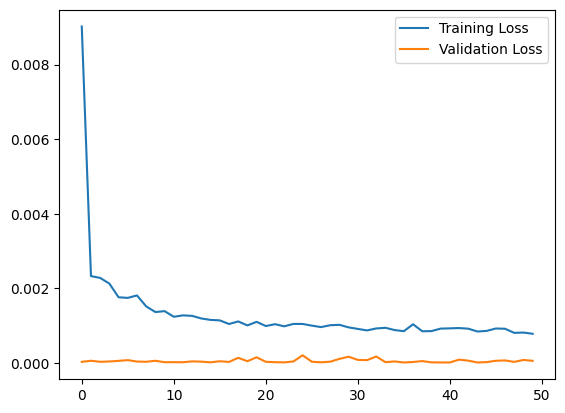
\includegraphics[width=0.8\linewidth]{Wyniki_testowe_i_walidacyjne.png}
    \caption{Wyniki testowe i walidacyjne}
    \label{fig:Wyniki_testowe_i_walidacyjne}
\end{figure}

\section{Bezpieczeństwo aplikacji}
Aplikacja wykorzystuje framework \texttt{Spring Security} w celu zapewnienia bezpieczeństwa i kontrolowania dostępu do zasobów. Dzięki zastosowaniu różnych mechanizmów uwierzytelniania i autoryzacji, takich jak \texttt{JWT} (JSON Web Tokens), oraz \texttt{Basic Authentication}, aplikacja jest chroniona przed nieautoryzowanym dostępem. Poniżej przedstawiono kluczowe komponenty zapewniające bezpieczeństwo aplikacji.\\[-10pt]

\noindent \textbf{Konfiguracja bezpieczeństwa (\texttt{SecurityConfig.java})~~}  
Pełną konfigurację bezpieczeństwa aplikacji zwiera klasa \texttt{SecurityConfig}. Definiuje ona ustawienia filtrów bezpieczeństwa, które kontrolują dostęp do zasobów. Endpointy \texttt{/client/register} i \texttt{/client/login}, służą użytkownikowi do rejestracji lub logowania, tak aby mógł mieć dostęp do platformy. 

Klasa ta zawiera również konfigurację \texttt{CORS}, która zezwala na dostęp do zasobów aplikacji z określonych domen (np. \texttt{http://localhost:3000}). Dzięki temu aplikacja ma możliwość komunikacji z frontendem.\\[-10pt]

\noindent \textbf{Generowanie i weryfikacja JWT (\texttt{JwtTokenUtils.java})~~} 
za generowanie oraz weryfikację tokenów \texttt{JWT} odpowiada klasa \texttt{JwtTokenUtils}. Tokeny te są wykorzystywane do uwierzytelniania użytkowników i zapewnienia im dostępu zasobów aplikacji. Klasa ta wykonuje następujące operacje:
\begin{itemize}
    \item Generowanie tokenów \texttt{JWT} z unikalnymi danymi użytkownika.
    \item Weryfikacja ważności tokenu, w tym sprawdzanie daty wygaśnięcia.
    \item Ustalenie, czy użytkownik w tokenie jest tym samym, który jest zapisany w bazie danych.
\end{itemize}
Po weryfikacji tokenu, użytkownik zostaje uwierzytelniony i przypisany do kontekstu bezpieczeństwa aplikacji.\\[-10pt]

\noindent \textbf{Filtrowanie tokenów JWT (\texttt{JwtAccessTokenFilter.java})~~} 
Za filtrację przychodzących żądań HTTP jest odpowiedzialna klasa \texttt{JwtAccessTokenFilter}. Filtr ten sprawdza nagłówek \texttt{Authorization} w żądaniach, aby wyodrębnić i zweryfikować token \texttt{JWT}. Jeśli token jest ważny, uzyskuje dostęp do platformy. W przypadku, gdy token jest nieważny lub nie istnieje, aplikacja zwraca odpowiedź o statusie \texttt{UNAUTHORIZED}.\\[-10pt]

\noindent \textbf{Zarządzanie danymi użytkowników (\texttt{UserInfoManager.java})~~} 
Klasa \texttt{UserInfoManager} implementuje interfejs \texttt{UserDetailsService} i jest odpowiedzialna za załadowanie użytkownika z bazy danych na podstawie nazwy użytkownika. Metoda \texttt{loadUserByUsername} korzysta z repozytorium \texttt{ClientRepository}, aby odnaleźć użytkownika, a następnie dostarcza jego dane do kontekstu bezpieczeństwa aplikacji, co pozwala na uwierzytelnianie.\\[-10pt]

\noindent \textbf{Rekordy RSA (\texttt{RSAKeyRecord.java})~~} 
Klasa \texttt{RSAKeyRecord} przechowuje klucze RSA (publiczny i prywatny), które są wykorzystywane do weryfikacji i generowania tokenów \texttt{JWT}. Klucz publiczny jest używany do weryfikacji podpisu tokenu, natomiast klucz prywatny służy do jego generowania. Jest to istotny element systemu autoryzacji, zapewniający integralność i~bezpieczeństwo transmisji danych.\\[-10pt]

\noindent \textbf{Podstawowe uwierzytelnienie (\texttt{BasicAuthenticationSecurityConfiguration.java})}
Klasa \texttt{BasicAuthenticationSecurityConfiguration} wprowadza mechanizm podstawowego uwierzytelnienia.
	

% LITERATURA (zostanie wygenerowana automatycznie)
%UWAGA: bibliotekę referencji należy przygotować samemu. Dobrym do tego narzędziem jest JabRef.
%       JabRef oferuje jednak większą liczbę typów rekordów niż obsługuje BibTeX.
%       Proszę nie deklarować rekordów o typach nieobsługiwanych przez BibTeX.
%       Formatowania wykazu literatury i cytowań odbywać się ma zgodnie z zadeklarowanym stylem.
%       Zalecane są style produkujące numeryczne cytowania (w postaci [1], [2,3]).
%       Takim stylem jest np. plabbrv
\bibliographystyle{plabbrv}
%       Aby zapanować nad odstępami w wykazie literatury można posłużyć się poniższą komendą
\setlength{\bibitemsep}{2pt} % - zacieśnia wykaz
%       Pozycja Literatura pojawia się w spisie treści nieco inaczej niż spisy rysunków, tabel itp.
%       Aby zachować właściwe odstępy należy użyć poniższej komendy
\addtocontents{toc}{\addvspace{2pt}} % ustawiamy odstęp w spisie treści przed pozycją Literatura 
%       Nazwę pliku przygotowanej biblioteki wpisuje się bez rozszerzenia .bib
%       (linia poniżej załaduje rekordy z pliku "dokumentacja.bib")
\bibliography{dokumentacja}
\appendix

% Jeśli w pracy pojawiać się ma indeks, należy odkomentować poniższe linie
%%\chapterstyle{noNumbered}
%%\phantomsection % sets an anchor
%%\addcontentsline{toc}{chapter}{Indeks rzeczowy}
%%\printindex

\end{document}
